%%%%%%%%%%%%%%%%%%%%%%%%%%%%%%%%%%%%%%%%%%%%
%Set Document Type
%%%%%%%%%%%%%%%%%%%%%%%%%%%%%%%%%%%%%%%%%%%%
\documentclass[11pt, a4paper, titles]{report}  %Remove "twoside" for pdf version, keep for printing. 

%%%%%%%%%%%%%%%%%%%%%%%%%%%%%%%%%%%%%%%%%%%%
%Packages
%%%%%%%%%%%%%%%%%%%%%%%%%%%%%%%%%%%%%%%%%%%%
%\usepackage{MyStyle}
\usepackage{graphicx}
\usepackage{xspace}
\usepackage[svgnames]{xcolor}
\usepackage{longtable}
\usepackage{amsmath}     %!  setspace is used to control linepacing
%\usepackage[square]{natbib} %! needed for Harvard style of references.
\usepackage{enumerate}  %! used for the library form, but you might find 
\PassOptionsToPackage{hyphens}{url}\usepackage{hyperref}
\hypersetup{
    colorlinks=true,
    linkcolor=black,
    citecolor=black,
    filecolor=black,
    urlcolor=black}
\usepackage[a4paper,width=150mm,top=30mm,bottom=25mm]{geometry} %Remove "left=4cm" for pdf version, keep for printing. 
\usepackage{multicol}
\usepackage{amssymb}
\usepackage{afterpage}
\usepackage{rotating}
%%%%%%%%%%%%%%%%%%%%%%%%%%%%%%%%%%%%%%%%%%%%
% Handle special characters
%%%%%%%%%%%%%%%%%%%%%%%%%%%%%%%%%%%%%%%%%%%%
\usepackage{textgreek}
\usepackage{arabtex}
\usepackage{utf8}
\setcode{utf8}
\usepackage{tipa} % for \textgamma
\DeclareUnicodeCharacter{1E24}{\d{H}}      % uppercase
\DeclareUnicodeCharacter{1E25}{\d{h}}      % lowercase
\DeclareUnicodeCharacter{0263}{\textgamma} 
%%%%%%%%%%%%%%%%%%%%%%%%%%%%%%%%%%%%%%%%%%%%
%References
%%%%%%%%%%%%%%%%%%%%%%%%%%%%%%%%%%%%%%%%%%%%
\usepackage[backend=bibtex, style=authoryear]{biblatex}
\addbibresource{NewTools.bib} %Import the bibliography file
\urlstyle{same}
%%%%%%%%%%%%%%%%%%%%%%%%%%%%%%%%%%%%%%%%%%%%
%Appendix
%%%%%%%%%%%%%%%%%%%%%%%%%%%%%%%%%%%%%%%%%%%%
\usepackage[toc,page]{appendix}
%%%%%%%%%%%%%%%%%%%%%%%%%%%%%%%%%%%%%%%%%%%%
%Footnotes
%%%%%%%%%%%%%%%%%%%%%%%%%%%%%%%%%%%%%%%%%%%%
\usepackage{scrextend}
%%%%%%%%%%%%%%%%%%%%%%%%%%%%%%%%%%%%%%%%%%%%
%Set Tables
%%%%%%%%%%%%%%%%%%%%%%%%%%%%%%%%%%%%%%%%%%%%
\usepackage{lscape}
\usepackage{tablefootnote}
\usepackage{array}
\usepackage{bigfoot}
\usepackage{booktabs}
\usepackage{threeparttablex}
\usepackage{multirow} 
% Add this line for caption customization
%%%%%%%%%%%%%%%%%%%%%%%%%%%%%%%%%%%%%%%%%%%%
%Acronyms
%%%%%%%%%%%%%%%%%%%%%%%%%%%%%%%%%%%%%%%%%%%%
\usepackage{acro}[=v2]
%%%%%%%%%%%%%%%%%%%%%%%%%%%%%%%%%%%%%%%%%%%%
%Chemistry
%%%%%%%%%%%%%%%%%%%%%%%%%%%%%%%%%%%%%%%%%%%%
\usepackage{chemformula}
%%%%%%%%%%%%%%%%%%%%%%%%%%%%%%%%%%%%%%%%%%%%
%Set Font
%%%%%%%%%%%%%%%%%%%%%%%%%%%%%%%%%%%%%%%%%%%%
\usepackage[onehalfspacing]{setspace}
\usepackage[scaled]{helvet}
\renewcommand\familydefault{\sfdefault} 
\usepackage[T1]{fontenc}
%\usepackage{newpxtext,newpxmath}
%Set section headers to not be bold
\usepackage[titles]{tocloft} %, calc}
%\renewcommand{\cftsecfont}{\mdseries}
%\renewcommand{\cftsecpagefont}{\mdseries}
%%%%%%%%%%%%%%%%%%%%%%%%%%%%%%%%%%%%%%%%%%%%
%Set Figure and Table Caption colour
%%%%%%%%%%%%%%%%%%%%%%%%%%%%%%%%%%%%%%%%%%%%
\usepackage{caption}
\usepackage{subcaption} 
\captionsetup[table]{labelsep=period, labelfont={bf}, font={small, stretch=1.5}}     %% change 1.2 as you like
\captionsetup[figure]{labelsep=period, labelfont={bf}, font={small, stretch=1.5}}
\captionsetup{width=0.98\textwidth}
%%%%%%%%%%%%%%%%%%%%%%%%%%%%%%%%%%%%%%%%%%%%
%Set Code Block Formatting
%%%%%%%%%%%%%%%%%%%%%%%%%%%%%%%%%%%%%%%%%%%%
\usepackage{listings}
\usepackage{color}
%%%%%%%%%%%%%%%%%%%%%%%%%%%%%%%%%%%%%%%%%%%
%Chapter Style
%%%%%%%%%%%%%%%%%%%%%%%%%%%%%%
\usepackage{epigraph} %To add quotes
\usepackage{titlesec}
\usepackage[normalem]{ulem}

\makeatletter
\def\@makechapterhead#1{%
    \vspace*{2em}% Space above number
    {\parindent \z@  \normalfont
    \interlinepenalty\@M
    \Huge\centering{\bfseries{\scshape Chapter\ \thechapter }}%
    \par\vspace{-2.63em}%
    \par\rule{.33\textwidth}{0.8pt}
    \par\vspace{0em}% Space between number and title
    \singlespacing\textbf{#1}%
    \par\vspace{1em}% Space between title and text
}}
\makeatother

\titleformat*{\section}{\Large\bfseries}
\titleformat*{\subsection}{\large\bfseries}
\titleformat*{\subsubsection}{\normalfont\bfseries}

%Paragraph Style
%%%%%%%%%%%%%%%%%%%%%%%%%%%%%%
\onehalfspacing
\usepackage{blindtext}
\usepackage{lastpage}
\usepackage{fancyhdr}
\usepackage{parskip}
\setlength{\parindent}{3em}

%Header and Footer Style
%%%%%%%%%%%%%%%%%%%%%%%%%%%%%%
\usepackage{xcolor}
\definecolor{headergray}{RGB}{128,128,128} % Define the grey color
\renewcommand{\headrule}{\textcolor{headergray}{\rule{\headwidth}{0pt}}} % Change the color of the header rule
\pagestyle{fancy}
\renewcommand{\sectionmark}[1]{\markboth{#1}{}}
\fancyhf{}
%\fancyhead[L]{\textcolor{headergray}{\small New Tools Thesis - Draft 1}}
\fancyhead[R]{\ifnum\value{chapter}=0\else\textcolor{headergray}{\small\chaptername~\thechapter  | \fi\leftmark}}
\fancyfoot{}
\fancyfoot[C]{\thepage}
%Prevent footnotes from breaking over multiple pages. 
\interfootnotelinepenalty=10000

%%%%%%%%%%%%%%%%%%%%%%%%%%%%%%%%%%%%%%%%                             
%Contents page
%%%%%%%%%%%%%%%%%%%%%%%%%%%%%%%%%%%%%%%%
\renewcommand{\cftchappresnum}{Chapter }
\AtBeginDocument{\addtolength\cftchapnumwidth{\widthof{\bfseries Chapter }}}

%%%%%%%%%%%%%%%%%%%%%%%%%%%%%%%%%%%%%%%%                             
%Acronyms
%%%%%%%%%%%%%%%%%%%%%%%%%%%%%%%%%%%%%%%%
                            
%Organism Names
%%%%%%%%%%%%%%%%%%%%%%%%%%%%%%%%%%%%%%%%

\DeclareAcronym{Fo}{
  short = \textit{Fo},
  long  = \textit{Fusarium oxysporum},
}

\DeclareAcronym{Focub}{
  short = \textit{Focub},
  long  = \textit{Fusarium oxysporum} f. sp. \textit{cubense}}

\DeclareAcronym{Focub4}{
  short = \textit{Focub} TR4,
  long  = \textit{Fusarium oxysporum} f. sp. \textit{cubense} Tropical Race 4}

\DeclareAcronym{Focub1}{
  short = \textit{Focub} R1,
  long  = \textit{Fusarium oxysporum} f. sp. \textit{cubense} Race 1,
}

\DeclareAcronym{Foly}{
  short = \textit{Foly},
  long  = \textit{Fusarium oxysporum} f. sp. \textit{lycopersici},
}

\DeclareAcronym{Fon}{
  short = \textit{Foni},
  long  = \textit{Fusarium oxysporum} f. sp. \textit{niveum},
}

\DeclareAcronym{Fona}{
  short = \textit{Fona},
  long  = \textit{Fusarium oxysporum} f. sp. \textit{narcissi},
}

\DeclareAcronym{Fola}{
  short = \textit{Fola},
  long  = \textit{Fusarium oxysporum} f. sp. \textit{lactucae},
}

\DeclareAcronym{Foci}{
  short = \textit{Foci},
  long  = \textit{Fusarium oxysporum} f. sp. \textit{coriandrii},
}

\DeclareAcronym{Foma}{
  short = \textit{Foma},
  long  = \textit{Fusarium oxysporum} f. sp. \textit{matthiolae},
}

\DeclareAcronym{Foa}{
  short = \textit{Foap},
  long  = \textit{Fusarium oxysporum} f. sp. \textit{apii},
}

\DeclareAcronym{Fs}{
  short = \textit{Fs},
  long  = \textit{Fusarium sacchari},
}

\DeclareAcronym{Fm}{
  short = \textit{Fm},
  long  = \textit{Fusarium mindanaoense},
  mark-as-used=first
}

\DeclareAcronym{Ff}{
  short = \textit{Ff},
  long  = \textit{Fusarium fujikuroi},
}

\DeclareAcronym{Fg}{
  short = \textit{F. graminearum},
  long  = \textit{Fusarium graminearum},
}

\DeclareAcronym{r1}{
  short = R1,
  long  = Race 1,
}

\DeclareAcronym{r2}{
  short = R2,
  long  = Race 2,
}  

\DeclareAcronym{r3}{
  short = R3,
  long  = Race 3,
}  

\DeclareAcronym{r4}{
  short = R4,
  long  = Race 4,
}

\DeclareAcronym{tr4}{
  short = TR4,
  long  = Tropical Race 4,
}

\DeclareAcronym{str4}{
  short = STR4,
  long  = Sub-Tropical Race 4,
}

\DeclareAcronym{fsp}{
  short = f. sp.,
  short-plural-form = f. spp.,
  long = \textit{forma specialis},
  long-plural-form  = \textit{formae speciales},
}

\DeclareAcronym{FFSC}{
  short = FFSC,
  long  = \textit{Fusarium fujikuroi} species complex,
}  

\DeclareAcronym{FOSC}{
  short = FOSC,
  long  = \textit{Fusarium oxysporum} species complex,
} 

\DeclareAcronym{FGSC}{
  short = FGSC,
  long  = \textit{Fusarium graminearum} species complex,
} 

\DeclareAcronym{vcg}{
  short = VCG,
  long  = Vegetative Compatibility Group,
} 

\DeclareAcronym{xvm}{
  short = \textit{Xvm},
  long  = \textit{Xanthomonas vasicola} pv. \textit{musacearum},
} 

\DeclareAcronym{fwb}{
  short = FWB,
  long  = Fusarium wilt of banana} 

  \DeclareAcronym{xwb}{
  short = XWB,
  long  = Xanthomonas wilt of banana,
} 

%Genes, Proteins etc
%%%%%%%%%%%%%%%%%%%%%%%%%%%%%%%%%%%%%%%%
\DeclareAcronym{tef}{
  short = TEF-1\textalpha,
  long  = translation elongation factor-1\textalpha ,
}

\DeclareAcronym{rbp2}{
  short = RPB\textit{ii},
  long  = RNA polymerase subunit 2,
}

\DeclareAcronym{mites}{
  short = MITEs,
  long  = Miniature inverted-repeat transposable elements,
}

\DeclareAcronym{te}{
  short = TE,
  long  = transposable element,
}

\DeclareAcronym{mimp}{
  short = \textit{mimp},
  long  = \textit{\underline{m}iniature \underline{imp}ala},
}

\DeclareAcronym{sixg}{
  short = \textit{SIX} gene,
  long  = \textit{Secreted In Xylem} gene,
}

\DeclareAcronym{sixp}{
  short = SIX protein,
  long  = Secreted In Xylem protein,
}

\DeclareAcronym{vic}{
  short = \textit{Vic},
  long  = \textit{Vegetative Incompatibility}}

\DeclareAcronym{rga2}{
  short = \textit{RGA2},
  long  = \textit{Resistance Gene Analog 2}}



%Biologial Processes & General Terms
%%%%%%%%%%%%%%%%%%%%%%%%%%%%%%%%%%%%%%%%
\DeclareAcronym{AVR}{
short = AVR,
long = avirulence,
}

\DeclareAcronym{cec}{
short = CEC,
long = candidate effector cluster}

\DeclareAcronym{ce}{
short = CE,
long = candidate effector,
}

\DeclareAcronym{mimpce}{
short = MACE,
long = \textit{mimp}-associated candidate effector,
}

\DeclareAcronym{ac}{
short = AC,
long = accessory chromosome,
}

\DeclareAcronym{cc}{
short = CC,
long = core chromosome,
}

\DeclareAcronym{bp}{
short = bp,
long = base pair,
}

\DeclareAcronym{tir}{
short = TIR,
long = Terminal Invert Repeat,
}

\DeclareAcronym{prr}{
short = PRRs,
long = pattern recognition receptors,
}

\DeclareAcronym{nlr}{
short = NLR,
long = nucleotide-binding leucine-rich receptor,
}

\DeclareAcronym{pamp}{
short = PAMPs,
long = pathogen-associated molecular patterns,
}

\DeclareAcronym{pti}{
short = PTI,
long = PAMP-triggered immunity,
}


\DeclareAcronym{pcr}{
short = PCR,
long = polymerase chain reaction,
}
  
\DeclareAcronym{eti}{
short = ETI,
long = effector-triggered immunity,
}

\DeclareAcronym{ets}{
short = ETS,
long = effector-triggered susceptibility,
}

\DeclareAcronym{rprot}{
short = R proteins,
long = resistance proteins,
}

\DeclareAcronym{rgene}{
short = R gene,
long = resistance gene,
}

\DeclareAcronym{nafld}{
short = NAFLD,
long = Non-Alcoholic Fatty Liver Disease,
}

\DeclareAcronym{nafl}{
short = NAFL,
long = Non-Alcoholic Fatty Liver,
}

\DeclareAcronym{nash}{
short = NASH,
long = Non-Alcoholic Steato-Hepatitis,
}
                   
%Bioinf 
%%%%%%%%%%%%%%%%%%%%%%%%%%%%%%%%%%%%%%%%
\DeclareAcronym{blast}{
short = BLAST,
long = Basic Local Alignment Tool,
}

\DeclareAcronym{orf}{
short = ORF,
long = Open Reading Frame,
}

\DeclareAcronym{busco}{
short = BUSCO,
long = Benchmarking Universal Single-Copy Orthologs,
}

\DeclareAcronym{maei}{
short = MAEI,
long = \textit{Mimp}-Associated Effector Identification,
}

\DeclareAcronym{star}{
short = STAR,
long = Spliced Transcripts Alignment to a Reference,
}

\DeclareAcronym{ml}{
short = ML,
long = machine learning,
}

\DeclareAcronym{phibase}{
short = PHI-base,
long = Pathogen-Host Interaction Database,
}               

%Stats
%%%%%%%%%%%%%%%%%%%%%%%%%%%%%%%%%%%%%%%%
\DeclareAcronym{anova}{
short = ANOVA,
long = Analysis of Variance,
}

\DeclareAcronym{plsda}{
short = PLS-DA,
long = Partial Least Squares-Discriminant Analysis,
}

\DeclareAcronym{hmm}{
short = HMM,
long = Hidden Markov Model
}

\DeclareAcronym{fc}{
short = FC,
long = fold change
}



%Experimental Terms and Techniques
%%%%%%%%%%%%%%%%%%%%%%%%%%%%%%%%%%%%%%%%

\DeclareAcronym{hpi}{
short = hpi,
long = hours post-inoculation,
}

\DeclareAcronym{dpi}{
short = dpi,
long = days post-inoculation,
}

\DeclareAcronym{wpi}{
short = wpi,
long = weeks post-inoculation,
}

\DeclareAcronym{ont}{
short = ONT,
long = Oxford Nanopore Technologies,
}

\DeclareAcronym{hplc}{
short = HPLC,
long = high-performance liquid chromatography,
}

\DeclareAcronym{lcms}{
short = LC-MS,
long = Liquid Chromatography-Mass Spectrometry,
}

\DeclareAcronym{esi}{
short = ESI,
long = electrospray ionisation,
}

\DeclareAcronym{lamp}{
short = LAMP,
long = Loop-mediated isothermal amplification
}

\DeclareAcronym{pda}{
short = PDA,
long = potato dextrose agar,
}

\DeclareAcronym{pdb}{
short = PDB,
long = potato dextrose broth,
}

\DeclareAcronym{ypgb}{
short = YPGB,
long = {yeast, peptone, and glucose broth},
}

\DeclareAcronym{ypga}{
short = YPGA,
long = {yeast, peptone, and glucose agar},
}

\DeclareAcronym{rpm}{
short = rpm,
long = revolutions per minute
}

\DeclareAcronym{sdw}{
short = SDW,
long = sterile distilled water
}

\DeclareAcronym{um}{
short = UM,
long = untargeted metabolomics,
}

\DeclareAcronym{srm}{
short = SRM,
long = selected reaction monitoring,
}

%Organisations
%%%%%%%%%%%%%%%%%%%%%%%%%%%%%%%%%%%%%%%%
\DeclareAcronym{FAO}{
short = FAO,
long = Food and Agriculture Organisation of the United Nations}

\DeclareAcronym{wbf}{
short = WBF,
long = World Banana Forum}

\DeclareAcronym{ncbi}{
short = NCBI,
long = National Center of Biotechnology Information}

\DeclareAcronym{ngdc}{
short = NGDC,
long = National Genomics Data Centre}

\DeclareAcronym{tnau}{
short = TNAU,
long = Tamil Nadu Agricultural University }

\DeclareAcronym{niab}{
short = NIAB,
long = National Institute of Agricultural Botany}


%Misc
%%%%%%%%%%%%%%%%%%%%%%%%%%%%%%%%%%%%%%%%

\DeclareAcronym{rs}{
short = RS,
long = remote sensing }

\DeclareAcronym{uav}{
short = UAV,
long = Unmanned Aerial Vehicle}

\DeclareAcronym{vi}{
short = VI,
long = Vegetation Indices}

\DeclareAcronym{ps2}{
short = PSII,
long = Photosystem II}




%%%%%%%%%%%%%%%%%%%%%%%%%%%%%%%%%%%%%%%%                             
%Start Document
%%%%%%%%%%%%%%%%%%%%%%%%%%%%%%%%%%%%%%%%
\linespread{2} 
\begin{document}

%%%%%%%%%%%%%%%%%%%%%%%%%%%%%%%%%%%%%%%%
%Title Pages
%%%%%%%%%%%%%%%%%%%%%%%%%%%%%%%%%%%%%%%%
\begin{titlepage}
\begin{titlepage}
    \begin{center}
        \singlespacing
        \Huge
        \textbf{New Tools for the Identification of} \\\vspace*{0.5cm} \textbf{\textit{Fusarium} Wilt in Banana} \\
        \vspace*{1.75cm}
        \normalsize
        by \\ 
        \vspace*{0.2cm}
        \LARGE
        Jamie Pike BSc (Hons) \\ 
        \vfill
        \normalsize
        Submitted in the partial fulfilment of the requirements for the degree of \\
        \Large
        \vspace*{0.3cm}
        Doctor of Philosophy in Life Sciences \\
        \vspace*{1cm}
        \includegraphics[width=0.4\textwidth]{Preamble/crest_black.eps} \\
        \vspace*{1cm}
        \large
        University of Warwick, School of Life Sciences\\
        \vspace*{0.5cm}
        \normalsize
        March 2024 \\
         \vspace*{1cm}   
    \end{center}
    \clearpage
\end{titlepage}
\end{titlepage}
\newpage
\pagestyle{empty} 

% %%%%%%%%%%%%%%%%%%%%%%%%%%%%%%%%%%%%%%%%
% %Quote
% %%%%%%%%%%%%%%%%%%%%%%%%%%%%%%%%%%%%%%%%
% \thispagestyle{empty} % Remove page number

% \begin{quote}
% \topskip0pt
% \vspace*{\fill}
% \raggedleft % Right-align text
% \textit{In nature, nothing exists alone.} \\
% \medskip
% -- Rachel Carson
% \end{quote}
% \vspace*{\fill}
% \thispagestyle{empty} 

%%%%%%%%%%%%%%%%%%%%%%%%%%%%%%%%%%%%%%%%
%Fromatting
%%%%%%%%%%%%%%%%%%%%%%%%%%%%%%%%%%%%%%%%
\newpage
\thispagestyle{empty} 

\pagenumbering{roman} %! Begins roman numerals start from page I.

\addtocontents{toc}{\protect\setlength{\cftbeforechapskip}{0pt}}

\setcounter{secnumdepth}{-2}% default for "report" is 2

%%%%%%%%%%%%%%%%%%%%%%%%%%%%%%%%%%%%%%%%
%Table of Contents
%%%%%%%%%%%%%%%%%%%%%%%%%%%%%%%%%%%%%%%%
\clearpage
\tableofcontents
\listoftables                     
\listoffigures  

%%%%%%%%%%%%%%%%%%%%%%%%%%%%%%%%%%%%%%%%
%Prelimary Sections
%%%%%%%%%%%%%%%%%%%%%%%%%%%%%%%%%%%%%%%%
\begin{spacing}{1}

\clearpage
\phantomsection
\addcontentsline{toc}{chapter}{Acknowledgements}
\chapter*{\huge\centering Acknowledgements}

First, I would like to thank my supervisor, Prof. Murray Grant. Murray has challenged me to become more independent, thoughtful, and confident as a researcher, and I am grateful for the support, guidance, time and wisdom he has provided. Second, I would like to thank Dr David Studholme for his valuable supervision and feedback, particularly in the race to finish this thesis. Next, I would like to thank Prof. John Clarkson and Dr Helen Bates. The opportunity to trial my pipeline on their \textit{Fusarium} genomes was invaluable, and the insights they provided were extremely useful. I would have a substantially smaller thesis without them. 

My thanks to Dr Laura Baxter for her advice, ideas, support and expertise. For every panicked error message I sent, Laura had sage advice. A huge thank you to Dr John Sidda. Not only must I thank John for the help he provided with all things metabolomic, but also for welcoming me to the group, his friendship, and his WhatsApp puns. My thanks to Dr Lijiang Song, Dr Zac Newland-Smith, and Nadine Aschuer for their help in processing many metabolomics samples. I also thank Dr Raveendran Muthurajan at TNAU. Of course, a big thank you to all the members of C46 and the Grant group, past and present. 

This PhD would not have been possible without the funding provided by the Waitrose CTP, I am grateful to the CTP for the financial support and the wider Waitrose CTP training opportunities and events. 

Beyond the PhD, I would like to thank (Dr) Annabelle de Vries and (Dr) Sadik Muzemil for their help, friendship, and opportunities to chat, brainstorm, and panic in B1.34. On the subject of helpful friends, I must thank Hannah and Alissa for the many, many hours they spent proofreading this thesis, as well as their encouragement and, occasionally welcome, cat-related distractions. I would like to thank Tash, Ciaran, Rosie, Harry, and Delenn, as well as Dr James Wagstaffe, Dr Rachel Kaleta, and Ms Melanie Webb, Dr Kevin King, Dr Jon West, and Ms Gail Canning for their horticultural and scientific enthusiasm. My thanks to Justine, Emma, Tommy, Nan and everyone Pike, Warren,  Fleckney, or otherwise, who has encouraged and supported me.  

Finally, a special thanks to my partner, Mark, whose unwavering love, support, and understanding has been invaluable. Additionally, I am deeply grateful to my parents for their endless love, encouragement, and the sacrifices they have made to support my academic pursuits. Their guidance, belief in me, and unwavering support have been fundamental to my success, and I am profoundly grateful for everything they have done. 






\clearpage
\phantomsection
\addcontentsline{toc}{chapter}{Thesis Declaration}
\chapter*{\huge\centering Thesis Declaration}
This thesis is submitted to the University of Warwick in support of my application for the degree of Doctor of Philosophy. It has been composed by myself and has not been submitted in any previous application for any degree. The work presented (including data generated and data analysis) was carried out by the author except in the cases outlined below. 
\noindent
\subsubsection{Data provided and/or analysis carried out by collaborators.}
\begin{itemize}
    \item Virulence assays and generation of genomic read data for \textit{Fusarium} isolates, S6, S16, S32, and SY-2. Data was supplied by Dr Raveendran Muthurajan and collaborators at \acl{tnau}. 
    \item Genome assemblies for some \acl{Fo} isolates (denoted in tablem\ref{tab:GenomeDB}) were supplied by Dr Helen Bates and collaborators at \acl{niab} and Prof. John Clarkson and group at the University of Warwick. 
    \item RNAseq data and supporting analysis for \acl{Fo} isolates (AJ516, AJ520, AJ705, AJ260, and Fo47) were supplied by Dr Helen Bates and collaborators at \acl{niab} and Prof. John Clarkson and group at the University of Warwick. 
    \item The \acl{tef} database used for phylogenetic analysis was compiled by Chloe Harper, as part of her undergraduate research project (supervised by Prof. John Clarkson, University of Warwick).
    \item Scripts used for IPO and XCMS analysis were supplied by Dr John Sidda, University of Oxford.
\end{itemize} 

\subsubsection{Publications including submitted papers.}
\begin{itemize}
    \item Parts of the analysis conducted in Chapter 2 have been submitted for publication, entitled: \textit{Comparative genomics and transcriptomics reveal differences in effector complement and expression between races of Fusarium oxysporum f.sp. lactucae}. 
\end{itemize}


\clearpage
\phantomsection
\addcontentsline{toc}{chapter}{Abstract}
\chapter*{\huge\centering Abstract}
Bananas (Musa spp.) are one of the world’s top agricultural commodities, but global banana production is threatened by \acf{fwb}. Historically caused by \acf{Focub}, \acf{fwb} devastated the global production of ‘Gros Michel’ in the 1900s, only to be saved by the resistant Cavendish sub-group. Cavendish bananas are susceptible to an emerging race of \acf{Focub}, \ac{tr4}, and, since its identification, \ac{Focub4} has spread internationally. Now present in Asia, Africa, Australia, Europe, and South America. 

\textit{Fusarium} isolates pathogenic towards Cavendish banana were collected by collaborators at \acf{tnau} and raw sequence data was shared. Subsequent phylogenetic analysis and virulence gene profiling suggest that two of the isolates shared are from the \acl{FFSC}, and closely related to \acl{Fs}. Further, our data suggest a third isolate is from the newly recorded species, \acl{Fm} sp. nov \parencite{Nozawa2023}. 

We also compiled a database of publicly available \acf{Fo} genomes and recently sequenced genomes of isolates pathogenic towards lettuce, celery, and coriander\footnote{in collaboration with Prof. John Clarkson, University of Warwick and Dr Helen Bates, \acl{niab}}. We developed a computational pipeline for novel virulence gene discovery using a family of commonly associated, short (~180bp) transposable elements, known as \aclp{mimp} \parencite{Schmidt2013}. For the \ac{Fo} genomes included in our analysis, we identified host-specific candidate effector profiles, including novel candidate effectors.

Finally, we the first employed \acl{um} to investigate banana interactions with \ac{Focub} and aid in the development of diagnostics. We identified features of interest that appeared to distinguish three different wilting stresses (\ac{fwb}, \textit{Xanthomonas} wilt of banana, and drought stress). These unique features of interest can be explored as putative biomarkers, and their role in wilt stress response investigated. 

Our interdisciplinary approach has advanced our understanding of \ac{fwb} and its interaction with banana. We have provided insights into pathogen diversity and virulence mechanisms in \ac{fwb}. The findings of this thesis highlight the urgency of ongoing surveillance and diagnostic development to combat \ac{fwb}, as well as the broader applicability of our methodologies in plant disease management. 


\clearpage
\phantomsection
\addcontentsline{toc}{chapter}{Abbreviations}
\chapter*{\huge\centering Abbreviations}  
\printacronyms[heading=none]
\clearpage

\end{spacing}

\setcounter{secnumdepth}{2}


%%%%%%%%%%%%%%%%%%%%%%%%%%%%%%%%%%%%%%%%%%%%
%Main Chapters
%%%%%%%%%%%%%%%%%%%%%%%%%%%%%%%%%%%%%%%%
\renewcommand{\arraystretch}{1.5} %Extend tables so they're easier to read
%Set chapter names and .tex files with chapter content.    
\pagestyle{fancy} 

\chapter{General Introduction}\label{Chap1}
\chaptermark{Introduction}
\pagenumbering{arabic} %! Begins arabic numerals start from page 1.
    \section {An Introduction to Banana}

Banana (\textit{Musa} spp.) is frequently reported as one of the world’s top agricultural commodities. Annual global production of bananas (including plantain) steadily increased from 98.4 million tonnes in 2000 to an estimated 155.2 million tonnes in 2018 (\ac{FAO}, 2020). A staple food and cash crop of significant agricultural, financial, and social importance, only around 15\% of bananas produced worldwide are traded in international markets, the remaining 85\% are consumed locally (\ac{FAO}, 2018), highlighting the value of bananas as a subsistence crop. Particularly in developing countries where fruits can account for 25\% of daily calorie intake and act as a source of income (\ac{FAO}, 2018).

\subsection{Anatomy and Classification of Banana}  

Banana is a monocotyledonous, herbaceous perennial which belongs to the Musaceae family in the order Zingiberales (Table ~\ref{tab:TaxonTable}) (Schoch \et 2020). Currently, there are 74 species of \textit{Musa} accepted by the World Checklist of Selected Plant Families (WCSP, 2022), including wild, ornamental, and cultivated species. Linnaeus originally described two species of banana: \textit{M. sapientum }and \textit{M. paradisiaca}. However, the classification of banana using the formalised binomial system following Linnaeus proved ineffective due to banana’s complicated genetic history (Cheesman, 1947).  

% Please add the following required packages to your document preamble:
% \usepackage{longtable}
% Note: It may be necessary to compile the document several times to get a multi-page table to line up properly
\begingroup
\setlength{\tabcolsep}{15pt} % Default value: 6pt
\renewcommand{\arraystretch}{0.9}
\begin{longtable}[c]{cc}
\caption[Taxonomy of \textit{Musa} genus]{\textbf{Taxonomy of \textit{Musa} genus including 3 example species} (Schoch et al., 2020, WCSP, 2022).}
\label{tab:TaxonTable}\\
\hline
\textbf{Kingdom}     & Plantae       
\endfirsthead
%
\multicolumn{2}{c}%
{{\bfseries Table \thetable\ continued from previous page}} \\
\endhead
%
\textbf{Phylum}      & Tracheophytes \\ 
\textbf{Class}       & Magnoliopsida \\ 
\textbf{Super order} & Lilianae      \\ 
\textbf{Order}       & Zingiberales  \\ 
\textbf{Family}      & Musaceae      \\ 
\textbf{Genus}       & \textit{Musa} \\ 
\textbf{Species} & \textit{\begin{tabular}[c]{@{}c@{}}M. acuminata,\\
M. balbisiana, \\
M. basjoo\end{tabular}} \\ \hline
\end{longtable}
\endgroup

In the mid-20th century, Cheesman, (1947) recognised the two species described by Linnaeus to be cultivars of wild the \textit{Musa} species \textit{M. acuminata }and \textit{M. balbisiana} and regrouped the remaining \textit{Musa} species into 4 ‘sections’. Building on the work of Cheesman, Simmonds and Shepherd, (1955) developed a genome-based, informal nomenclature system for cultivated banana which is still used today. The system classifies varieties into genome groups based on the ploidy contribution of their wild ancestors, where the species contribution is denoted by the letters ‘A’ and ‘B’ for \textit{M. acuminata} and \textit{M. balbisiana}, respectively. For example, “Cavendish banana (\textit{Musa }spp. AAA group) cv. ‘Grand Nain’” indicates the variety’s sub-group (Cavendish), genus (\textit{Musa}), genome group scoring (AAA), and cultivar (Grand Nain).

The anatomy of banana plants is outlined in detail by Robinson and Saúco, (2010) and Bakry \et (2009). Briefly, plants produce a fibrous root system from a tuberous rhizome. Extended horizontal growth, typical of most rhizomatous plants, is not observed in banana; the plant instead produces suckers which successively grow outwards from the short rhizome. The leaves are produced from the central meristem of the rhizome, or developing sucker, and laminae continue to widen until they mature. As leaf sheaths develop, they become tightly packed and thicken to form the pseudostem which elongates as more leaves emerge to 1-8m in height (Bakry \et 2009) (Figure ~\ref{fig:Anatomy of fruiting banana plant}). 

\begin{figure}[hp]
    \centering
    \includegraphics[width=12cm]{Figures/Diagrammatic-representation-of-a-fruiting-banana-plant-with-suckers-in-Bakry-et-al_W640.jpg}
    \caption[Anatomy of fruiting banana plant]{\textbf{Anatomy of fruiting banana plant} (From Bakry, et al. (2009)).}
    \label{fig:Anatomy of fruiting banana plant}
\end{figure}

\subsection{The History, Cultivation, and Value of Banana}

Originating from Southeast Asia, naturally occurring parthenocarpic – development of fruit without fertilisation – individuals of banana have been cultivated for about 10,000 years. Evidence of this can been seen in \textit{Musa banksii} phytoliths discovered in the Kuk swamp in Papua New Guinea (Denham, 2011). Cultivated bananas were spread from Papua New Guinea, hybridising with other subspecies of \textit{M. acuminata} and \textit{M. balbisiana} in the Philippines and northern New Guinea (Perrier \et 2009). Triploid cultivars were produced as a consequence and were dispersed throughout Southeast Asia, Northern Australia, East Africa, and South Asia by the Austronesian peoples; where, although primarily cultivated as a food crop, banana was used in traditional medicine to treat ailments including dysentery, ulcers, leprosy, epilepsy and insect bites (Kumar \et 2012). In these regions, banana has also been used as fodder; in domestic materials, such as plates, children’s toys and dyes; in building for shelter, rafts, or rope; and has significant social and cultural value, involved in many traditional rituals and customs (Hapsari \et 2017).  

Banana cultivation continued to move into the Middle East and Northern Africa from the centre of domestication in Southeast Asia, which can be seen in references banana in Islamic texts such as Ibn al-'Awwam's 12th-century agricultural work, Book on Agriculture (Clément-Mullet, 1866). During expeditions in Southeast Asia and Africa in the mid-1500s, bananas were encountered by Europeans (Amano \et 2021) who transported plants to South America where colonists established banana plantations to supply the USA and Europe (Guzmán-Rivas, 1960, Salas-Pascual and Cáceres-Lorenzo, 2022). This legacy continues today, with over 70\% of the EU’s banana supply coming from South American countries (EuropeanUnion, 2022).  

Banana production takes place year-round in tropical and subtropical regions, where plants are commercially grown as a monoculture crop. Plants are also cultivated by smallholders and in subsistence production systems (Viljoen \et 2020). Commercially, fruits are harvested within about 9-12 months of planting (either\textit{ in vitro} propagated material or suckers) and are grown as a ratoon crop – the plant is cut back to the rhizome once the fruit has been harvested and left to regrow – for several years, by which time yields will have reduced and a new plantation must be generated (BananaLink, 2020). The world’s largest banana growers are India and China which produced over 30 million tonnes and 11 million tonnes in 2018, respectively.  Currently, up to 40\% of all global banana production (domestic and export markets) is reliant on the Cavendish bananas (Warman and Aitken, 2018), a triploid, clonally propagated subgroup deriving from \textit{M. acuminata}. 

\subsection{Bananageddon! \textit{\acl{Fo}} and Current Banana Production}

In recent decades, there have been increasing reports of a potential ‘Bananageddon!’, whereby global banana production is decimated by the soil-borne, fungal pathogen \acl{Focub} (\ac{tr4}), the causative agent of Fusarium wilt of banana (syn. Panama disease). The global banana community’s concern is reflected in the establishment of the \ac{tr4} Task Force as part of the \ac{FAO}'s \ac{wbf}, the Peruvian government’s decision to declare a National Emergency upon the discovery of \ac{Focub} \ac{tr4} in 2021 (FAO, 2021), and in the recent publication by van Westerhoven \et (2022), where the authors stress the threat \ac{Focub} poses to African food security.   

\section{An Introduction to \acl{Focub}}

\subsection{A Brief History of Fusarium Wilt}

The robust response to \ac{Focub4} s not unfounded. During the first half of the 20th century, \ac{Focub} \ac{r1} devastated global production until the resistant banana subgroup, Cavendish, was identified. \ac{Focub} \ac{r1} destroyed approximately 40,000 hectares of ‘Gros Michel’ plantations (Agrios, 2005), and resulted in estimated economic losses of \$400 million (USD) between 1940 and 1960 (Ploetz, 2005). \ac{Focub} \ac{r1} led to the disappearance of ‘Gros Michel’ as an export banana in the 1960s (Molina \et 2007).  

Cavendish bananas were identified as resistant to \ac{Focub} \ac{r1} and subsequently replaced ‘Gros Michel’ (Ordonez \et 2015). However, from the 1960s Cavendish banana plants in Taiwan were observed displaying symptoms of \ac{Focub} infection (Agrios, 2005). Identified in 1994 as \acl{Focub4} (Ploetz, 1994), the strain affecting Cavendish bananas has continued to spread. \ac{Focub4} is now found in Africa, Asia and Europe (Ploetz, 2015a, Thangavelu \et 2019) and is gaining a foothold in South America with recent incursions in Columbia in 2019 (Garcia-Bastidas \et 2019), Peru in 2021 (\ac{FAO}, 2021), and Venuzuela in 2023 (Herrera, \et 2023).

\subsection{Disease Development of \acl{Focub}}

As a soil-borne pathogen, \ac{Focub} first colonises the roots. Asexual spores found in the soil germinate in response to host root exudates. Infection hyphae produced from resting spores (chlamydospores) penetrate the root epidermis at the tip. \ac{Focub} hyphae progress through the root cortex to the rhizome. \ac{Focub} migrates through the xylem in the outer leaf sheaths of the pseudostem occluding vessels and interferes with nutrient uptake and upward water transport; often before external symptoms are observed (Li \et 2017a, Warman and Aitken, 2018). Two asexual spore types, microconidia and macroconidia, are produced within the xylem and help \ac{Focub} overcome some of the host’s barriers, such as naturally occurring end walls or perforation plates of the xylem strands which somewhat inhibit pathogen movement through the host (Dita \et 2018). Xylem vessels begin to collapse, and external symptoms are observed. Tissues become chlorotic and the plant withers as it transpires more than it can translocate. Once the plant dies, the fungus begins to invade other plant tissues and sporulate, particularly on the plant surface, producing chlamydospores (Figure ~\ref{fig:MyLifeCylce}). Chlamydospores can persist in the soil for decades and are resistant to adverse conditions (Pegg \et 2019).  

\begin{figure}[hp!]
    \centering
    \includegraphics[width=14cm]{Figures/MyLifeCylceNarrow.pdf}
    \caption[Fusarium wilt of banana disease cycle.]{\textbf{Fusarium wilt of banana disease cycle.} Chlamydospores germinate in the soil in response to plant root exudates. Infection hyphae from Chlamydospores penetrate the root tip epidermal cells and progress through then host root cortex to the xylem. Microconidia and macroconidia are produced in the xylem and help to facilitate pathogen movement through the host. As Foc migrates through the xylem it occludes vessels and interferes with nutrient uptake and upward water transport. External wilting symptoms begin to develop; tissues become chlorotic and the plant withers as it transpires more than it can translocate. Eventually, the plant dies, and asexual spores are formed on the dead tissue. Chlamydospores persist in the soil or Foc survives endophytically in an alternative host species. Fungal hyphae are shown in blue. Images of Foc spores adapted from Fourie \et  (2011) and symptomatic banana plant images sourced from Maymon \et  (2020). Figure created with BioRender.com.}
    \label{fig:MyLifeCylce.}
\end{figure}


Alternative hosts, including many grass and weed species, also act as a reservoir of inoculum (Hennessy \et 2005).  \ac{Focub} is dispersed through the movement of contaminated plant and soil material, water, wind, and people. Typical symptoms of \ac{Focub} infection include pseudostem splitting and discolouration, yellowing of lower leaves often forming a ‘skirt’ around the plant, and, occasionally, a streaking pattern is observed on the foliage (Figure ~\ref{fig:FusariumWiltSymptoms}). 

\begin{figure}[hpt!]
    \centering
    \includegraphics[width=15cm]{Figures/SymptomsofFoc.pdf}
    \caption[Typical symptoms of Fusarium  wilt of banana.]{\textbf{Typical symptoms of \textit{Fusarium} wilt of banana.} (a) Splitting of the psuedostem, (b) discolouration of the psuedostem, (c) yellowing of lower leaves, and (d), a streaking pattern is observed on the foliage.}
    \label{fig:FusariumWiltSymptoms}
\end{figure}

\subsection{Classification of \acl{Focub}}

\ac{Focub} belongs to the \ac{FOSC}. The species complex contains both plant and animal pathogens, as well as saprophytes and endophytes (Leslie and Summerell, 2006). \ac{Fo} has high functional and genetic diversity, shown plainly in its broad plant host range. The species complex can infect around 150 species of both monocotyledonous and dicotyledonous plants, including many horticulturally significant crops such as banana, tomato and lettuce  (Edel-Hermann and Lecomte, 2019).  Individual pathogenic \ac{Fo} isolates can infect only one or a few plant species. Plant pathogenic \ac{Fo} are therefore divided into ‘special forms’, or (\ac{fsp}), each of which is adapted to specific hosts (Snyder and Hansen, 1940). For instance, strains which cause Fusarium wilt in tomato are classified as \ac{Fol}. To date, 106 \ac{fsp} have been clearly described and with at least an additional 37 putative \ac{fsp} (Edel-Hermann and Lecomte, 2019).   

Some \ac{fsp} can be further subdivided into pathogenic races, determined by pathogenicity towards specific host cultivars. Three races of \ac{Focub} affecting banana have been identified. \acl{r1} affects banana cultivars such as ‘Gros Michel’ (AAA), ‘Maqueno’, ‘Silk’, ‘Pome’ (AAB), and ‘Pisang Awak’ (ABB); \acl{r2} affects ‘Bluggoe’ and other cooking bananas (ABB); Race 4 affects the subgroup Cavendish (AAA) as well as hosts of \ac{r1} and \ac{r2} (Ploetz, 2015a) and has been further divided into \ac{str4} (S\ac{tr4}) and  (\ac{tr4}). \ac{tr4} is distinguished from \ac{str4} as it affects susceptible cultivars without disease-predisposing conditions (Ploetz, 2015b).  

Identification of isolates based on race is often subjective. During the 1980s an additional method of \ac{Focub} identification based on \ac{vcg} was developed (Correll, 1991). \ac{vcg}s are comprised of isolates that possess the same alleles at all \ac{vic} loci, and so can form stable heterokaryons with each other (Correll, 1991). So far, 24 \ac{vcg}s of \ac{Focub} have been identified (Table ~\ref{tab:VCGTab}) (Czislowski \et 2018).  Some \ac{vcg}s of \ac{Focub} are taxonomically closer to other \ac{fsp} of \ac{Fo} than other \ac{Focub} \ac{vcg}s. This, coupled with distinct genetic lineages identified through phylogenetic analysis, has resulted in the recognition of a polyphyletic – taxonomic group including members from different ancestral lineages – evolutionary history for \ac{Focub} (Koenig \et 1997, Ploetz, 2006). 

Maryani \et (2019) recently revised the taxonomy of \ac{Focub}, generating the Fusarium of Banana Species Complex and proposing several new species. However, Torres-Bedoya \et (2021) have suggested that the revision is premature and that the data do not fully support the revision. There continues to be active debate surrounding \ac{Focub} classification and a clear, robust, universally accepted taxonomy has not yet been established. Race, although somewhat informal, remains the most widely accepted method of \ac{Focub} classification – whereby isolates are identified based on virulence towards specific host cultivars.  

%Insert the VCG table
% Please add the following required packages to your document preamble:
% \usepackage{longtable}
% Note: It may be necessary to compile the document several times to get a multi-page table to line up properly
\begingroup
\setlength{\tabcolsep}{10pt} % Default value: 6pt
\renewcommand{\arraystretch}{0.67}
\begin{longtable}[tc!]{ccc}
\caption[\acf{vcg} of \ac{Focub}]{{\textbf{\acf{vcg} of \ac{Focub}} and race (Czislowski \et 2018).} Cross-compatible VCGs can form VCG complexes.}
\label{tab:VCGTab}\\
\hline
\textbf{VCG} & \textbf{VCG   complex} & \textbf{Race}    \\ \hline
\endfirsthead
%
\multicolumn{3}{c}%
{{\bfseries Table \thetable\ continued from previous page}} \\
\endhead
%
0120  & 0120–01215           & STR4             \\
0121  &                      & R4               \\
0122  &                      & R4               \\
0123  &                      & R1               \\
0124  & 0124–0125–0128–01220 & R1,   R2         \\
0125  & 0124–0125–0128–01220 & R1, R2           \\
0126  &                      & R1               \\
0127  & No longer valid      & No longer valid  \\
0128  & 0124–0125–0128–01220 & R1,   R2         \\
0129  & 0129–01211           & STR4             \\
01210 &                      & R1               \\
01211 & 0129–01211           & STR4             \\
01212 &                      & Not   Identified \\
01213 & 01213–01216          & TR4              \\
01214 &                      & R2               \\
01215 & 0120–01215           & STR4             \\
01216 & 01213–01216          & TR4              \\
01217 &                      & R1               \\
01218 &                      & R1               \\
01219 &                      & Not identified   \\
01220 & 0124–0125–0128–01220 & R1               \\
01221 &                      & Not Identified   \\
01222 &                      & Not   Identified \\
01223 &                      & Not Identified   \\
01224 &                      & Not   Identified \\ \hline
\end{longtable}
\endgroup

\section{The \acl{Fo} genome} 

An emerging explanation for shared host specificity between different \ac{Fo} lineages relates to the compartmentalisation of the \acl{Fo} genome. A theory which has become increasingly prevalent in \acl{Fo} genomics since the publication of Comparative genomics reveals mobile pathogenicity chromosomes in Fusarium by Ma \et in 2010. The study explains that the \textit{Fusarium} genome can be organised into two parts containing either core chromosomes or accessory (lineage-specific/supernumerary) chromosomes and suggests that these accessory chromosomes can be horizontally transferred. A theory which has since been demonstrated in Fol (Vlaardingerbroek \et 2016a, Vlaardingerbroek \et 2016b, Li \et 2020a), \acl{Fo} f. sp. \textit{radicis-cucumerinum} (van Dam \et 2017) and \acl{Fo} f. sp. \textit{melonis} (Li \et 2020b). 

The 11 core chromosomes within the \acl{Fo} genome encode functions necessary for primary metabolism and reproduction (van Dam \et 2017).  The remaining accessory chromosomes, which vary in number among \ac{fsp}, are not required for primary metabolism and reproduction, contain secondary metabolite biosynthetic gene clusters, encode virulence genes such as effectors, and possess a high number of transposable elements (Ma \et 2010, Schmidt \et 2013, Witte \et 2021). The accessory chromosomes which are particularly important for virulence are referred to as pathogenicity chromosomes.  Pathogenicity chromosomes within \acl{Fo} are often characterised by the presence of effector genes (Ma \et 2010). Effectors are secreted proteins that play an essential role in fungal colonisation of plant hosts and plant immune responses (Lo Presti \et 2015).  

\subsection{Segmental Duplication Paper}

\subsection{The Plant Innate Immune System}

The plant’s innate immune system is comprised of two interconnect tiers which perceive and respond to pathogen infection (Han, 2019, Ngou \et 2022). The first tier recognises microbial- or \ac{pamp} which are slow-evolving, conserved molecules (such as the fungal cell wall component, chitin) using transmembrane \ac{prr} on the plant cell surface. Once \ac{pamp} have been recognised, \ac{pti} is induced (Jones and Dangl, 2006). \ac{pti} responses include numerous cell signalling events such as altered ion fluxes, the production of apoplastic reactive oxygen species, callose deposition, and transcriptional reprogramming (Figure:~\ref{fig:PlantImmuneSystem}) (Han, 2019, DeFalco and Zipfel, 2021). 

\begin{figure}[h!]
    \centering
    \includegraphics[width=14cm]{Figures/DoddsArticleModel.pdf}
    \caption[Overview of the plant immune system.]{\textbf{Overview of the plant immune system.} Pattern recognition receptors (PRRs) perceive microbial- pathogen-associated molecular patterns (MAMPs/PAMPs) and induce a PAMP-triggered immunity (PTI) response from the host. In order to overcome host cell defences, pathogens secrete small molecules known as effectors into the host cell, inducing effector-triggered susceptibility (ETS). Plants have adapted a family of resistance proteins (R proteins), which can perceive pathogen effectors (avirulence proteins) and stimulate an effector-triggered immunity (ETI) response from the plant host (From Dodds and Rathjen, 2010).}
    \label{fig:PlantImmuneSystem}
\end{figure}

To evade, suppress or interfere with \ac{pti} responses and establish infection, fungal pathogens secrete proteins termed ‘effectors’ into the host cell which results in \ac{{ets} (Jones and Dangl, 2006, Ngou \et 2022). To combat \ac{ets}, plants possess a suite of \ac{rprot} which perceive effectors (termed ‘\ac{avr} effectors’) and induce further immune responses termed \ac{eti} (Jones and Dangl, 2006). \ac{rprot} are conserved intracellular receptors of the \ac{nlr} class. The structure, function, and effector perception (direct or indirect) of \ac{rprot} is variable and often specific (see: Chen \et 2022, Wang \et 2022). Similarly, effectors are typically highly variable and specific to individual pathogens (Lo Presti \et 2015).  


\subsection{The \acl{Fo} Effectorome}

In the \ac{FOSC}, the only family of effectors so far identified are the \ac{sixg}. In total, 14 SIX proteins (SIX1 – SIX14) have been identified through mass spectrometry of infected tomato xylem sap and whole genome sequencing (Houterman \et 2007, Schmidt \et 2013).  All 14 \ac{sixg}s are found on the pathogenicity chromosome in \ac{Fol} (Ma \et 2010, Schmidt \et 2013), and studies have confirmed that \textit{SIX1, SIX2, SIX3, SIX5} and \textit{SIX6} are essential for conferring virulence in tomato, with  \textit{SIX4} (\textit{Avr1}), \textit{SIX3} (\textit{Avr2}) and \textit{SIX1} (\textit{Avr3}) all recognised by corresponding \ac{rprot} (called ‘I’ for Immunity) in tomato (Rep \et 2004, Houterman \et 2007, Lievens \et 2009, Takken and Rep, 2010, Gawehns \et 2014, Ma \et 2015).  

Since their discovery in \ac{Fol}, homologs of \ac{sixg}s have been identified in other \ac{fsp}, including \textit{cepae, conglutinans, fragariae, melonis, pisi, radicis-cucumerinum,} and \textit{vasinfectum} (Czislowski \et 2018). A further \textit{SIX} gene, (\textit{SIX15}) has been described by Simbaqueba \et (2018) in \acl{Fo} f. sp. \textit{physalis}, although \textit{SIX15} is not widely reported.  

In \ac{Focub}, homologs of \textit{SIX1, SIX2, SIX4, SIX6, SIX7, SIX8, SIX9}, and \textit{SIX13} have been identified (Czislowski \et 2018, An \et 2019), and \textit{SIX1} and \textit{SIX8} have been recognised in \ac{Focub} \ac{tr4} as essential for virulence through knockout mutants (Widinugraheni \et 2018, An \et 2019). Czislowski \et (2018) reported differences in the \ac{sixg} repertoire of \ac{Focub} \ac{r1} and R4 lineages and hypothesised that the differences in \ac{sixg} profiles contribute to the variability in the \ac{Focub} host cultivar range.  However, as the authors point out, \ac{sixg}s are unlikely to be the only set of effectors involved in host specificity, and state ‘it should be expected that novel and undiscovered effectors remain to be identified in the lineages of \ac{Focub}’ (Czislowski \et 2018 pp. 1168).  

Ma \et (2010) showed that the pathogenicity chromosomes in \ac{Fol}, have a high number of retro-elements, including the non-autonomous class II \ac{te}, \ac{mites}. A specific family of \ac{mites}, known as \ac{mimp}s, are found upstream of all known \ac{sixg} in \ac{Fol} (Schmidt \et 2013). Characterised by their \ac{tir} sequence and short length (180–220 \ac{bp}), Schmidt \et (2013) surmised that \textit{mimps} could be used for the prediction of effectors in \acl{Fo}, particularly \ac{sixg}s, a theory which was later demonstrated by van Dam \et (2016), van Dam and Rep, (2017) and (Armitage \et 2018). 

The hypothesis that effector profiles contribute to host specificity is reported for other \ac{fsp} (Achari \et 2021, Batson \et 2021) and is argued on the host species level for the \ac{FOSC} (van Dam \et 2016). With advances in genome sequencing and analysis, it is possible to identify new candidate effectors using common characteristics shared between known effectors in \ac{Fol}, in other \ac{fsp}.

\section{Control of \acl{Focub}}

There are few effective controls for \ac{Focub} in the wider environment. Chlamydospores can persist in the soil for decades and \ac{Focub} can invade non-host plants and survive as an endophyte, with grass and weed species acting as sources of inoculum (Pegg \et 2019). Biological control agents and fungicides have been investigated as a means of \ac{Focub} control. However, most of these are \textit{in vitro} and greenhouse assays which, although successful, are not practical or effective in-field. (Moses, 2016, Chan \et 2017, Dita \et 2018).  

As most commercial bananas are triploid and parthenocarpic conventional breeding for resistance is exceedingly challenging (Dale \et 2017b). One somaclonal variant of Cavendish, ‘Formosana’ is marketed as being resistant to \ac{tr4}, however, yields are slightly reduced due to its longer growth cycle and there have been reports of  ‘Formosana’ showing \ac{tr4} susceptibility in later field trials (Lee \et 2011, Dale \et 2017a). A further somaclonal variant, ‘Guijiao 9’, is also marketed as showing lower disease severity compared to conventional commercial Cavendish varieties such as ‘Williams’ (Sun \et 2019), but, the variety has only recently been released to the market and field trials outside of the region in which this variety was developed have not yet been conducted.  

Advances in genetic modification technologies have facilitated the development of two \ac{tr4}-resistant transgenic Cavendish lines (Dale \et 2017). One of these lines, ‘QCAV-4’ is currently undergoing regulatory approval in Australia (Lu, 2023). The transgenic 'QCAV-4' variety was generated by transforming \textit{M. acuminata }Cavendish cv. 'Grand Naine' (AAA subgroup) embryogenic cell suspensions (prepared from immature male flowers) using the centrifugation assisted \textit{Agrobacterium tumefaciens}-mediated method with \ac{rga2}.\ac{rga2} is a putative \ac{nlr}-type \ac{rgene} from a seedling of \textit{Musa acuminata} ssp. \textit{malaccensis} with resistance to \ac{Focub4}. However, the market for genetically modified crops within Europe is limited, although debate and legislation are currently under review and development. 

Gene-edited banana may be a more marketable alternative, particularly for Europe, and editing for disease resistance has been demonstrated in banana. Tripathi \et (2021) used CRISPR-Cas9 to make mutations to the downy mildew resistance 6 (DMR6) orthologue in banana, showing enhanced resistance to the bacterial pathogen \ac{xvm}, this approach may be applied to target a gene which could provide resistance to \ac{Focub}.  

\subsection{The Role of Diagnostics in Banana Disease Detection and Management}

Prevention of \ac{Focub} introduction has so far proven the most effective method of \ac{Focub} control on a large scale (Ploetz, 2015b), with management primarily focused on hygiene practices. Therefore, emphasis has been placed on the development of accessible, fast, and accurate diagnostic tools (Ordóñez \et 2019). Molecular and image-based diagnostics have both been developed to identify \ac{Focub}. However, many of the current image-based diagnostics are currently unable to distinguish Foc from other banana wilt pathogens, and the molecular assays struggle to accurately identify pathogenic races.  
 

\section{Advancements in tech for diagnosing plant diseases}
\subsection{genomics?}
\subsection{imaging?}
\subsection{metabolomics? Human diseases?}


\newpage
\section{Project Aims and Objectives}

The overall aim of this research is to develop tools for the detection of \acl{Focub} \ac{tr4} in banana and contribute towards understanding of \acl{Focub} classification, identification, and infection and banana responses. 

\begin{enumerate}
    \item Build tools which aid in the identification of targets for molecular diagnostics and contribute to our understanding of \ac{Focub}-banana interactions as well as the evolutionary history and classification of \ac{Focub}. 
    \item Develop molecular diagnostics which can be used to identify specific races of \acl{Fo}. \footnote{Due to challenges sourcing isolates and sequence information from collaborators in Tamil Nadu Agricultural University, India (TNAU), our effector identification tool cannot currently be validated using Foc. However, we are testing this tool using other \acl{Fo} \ac{fsp} with collaborators at NIAB and the University of Warwick.}
    \item Employ phenomics to investigate banana responses to \ac{Focub} infection and contribute to the development of image-based diagnostic techniques.  
    \item Develop novel -omics approaches to improve understanding of banana interactions with \ac{Focub}.  
\end{enumerate}

\newpage
\section{Thesis Structure}

\subsection{Chapter 2: Potential Novel \textit{Fusarium} Pathogen of Banana Identified} 

This chapter will review the comparative genome assembly and subsequent analysis performed on \textit{Fusarium} isolates collected by collaborators at Tamil Nadu Agricultural University in India. Phylogeny of isolates and geographic distribution will be discussed compared to publicly available genomes, and a potential novel species presented. 

\subsection{Chapter 3: Improving Genomic Tools for Identifying Virulence Factors in \textit{Fusarium oxysporum}} 

This chapter will chart the development of the \textit{Mimp} Associated Effector Identification (Maei) tool which identifies effectors in \acl{Fo}, and the implications effector profiles have on the classification and genome compartmentalisation of the FOSC. It will include new genome sequences from collaborators at UoW and NIAB. Effector presence, location, predicted structures, homology, expression, and potential function will be explored. 
These candidate effectors will be used in the development of molecular diagnostics, and the potential of the Maei tool in the development of \acl{Fo} \ac{fsp} race-specific diagnostics will be explored. 

\subsection{Chapter 4: Phenomics: Image-based Analysis of Banana Stresses}

Banana disease imaging will be conducted and discussed, exploring the technologies currently available for image-based disease detection in banana, how spectral data can distinguish stresses, and why different spectral patterns are observed. 
We will also explore CT and microscopy data, recording the internal development of symptoms and how this relates to multispectral data. This data will also be discussed in chapter 4. 

\subsection{Chapter 5: Metabolomics: The Banana-pathogen Metabolome}
Untargeted Metabolomics analysis will be performed on infected banana to help develop our understanding of the \acl{Focub} infection process and indicate how this may be related to patterns observed in image-based analysis. We also identify specific markers of infection from a variety of biotic and abiotic stresses. 

\subsection{Chapter 6: General Discussion}
This chapter will discuss the main results from the thesis and will draw overall conclusions. It will also consider areas for improvement and future work. 


 

 



 



 



 
    
\chapter{A potential Newly Described \textit{Fusarium} Pathogen of Banana Identified in India}\label{Chap2}
    %%%%%%%%%%%%%%%%%%%%%%%%%%%%%%%%%%%%%%%%%%%%%
%INTRODUCTION
%%%%%%%%%%%%%%%%%%%%%%%%%%%%%%%%%%%%%%%%%%%%%

\section{\textbf{DRAFT:}An Introduction to plant pathogenic Fusarium species}
No text here yet. 



\subsection{\textit{Fusarium} of banana}
\subsection{Isolates collected by Tamil Nadu Agricultural University}

- Set story with TNAU isolates and Fusarium in India then add justification for this work!

This chapter presents the assembly and analysis of the genomic characteristics of \textit{Fusarium} isolates (SY-2, S6, S16, and S32) obtained from highly virulent on Cavendish banana plants by collaborators at Tamil Nadu Agricultural University (TNAU). taxonomic identity and genetic diversity are assessed and suggest that S6 is a \Focub race 1 isolate, while SY-2, S16 and S32 belong to the\textit{ F. fujikuroi} species complex. Phylogenetic analysis and \textit{SIX} gene profiling supported these classifications. Further investigations are necessary to ascertain whether SY-2, S16 and S32 represent a novel species within the \textit{F. fujikuroi} complex. Additionally, bacterial contamination with \textit{Stenotrophomonas} species was detected in S6 and S32 isolates, warranting future studies to explore potential implications on banana pathogenicity.

%%%%%%%%%%%%%%%%%%%%%%%%%%%%%%%%%%%%%%%%%%%%%
%METHODS
%%%%%%%%%%%%%%%%%%%%%%%%%%%%%%%%%%%%%%%%%%%%%

\section{Materials and Methods}
\subsection{Phenotyping and genotyping data supplied by TNAU.}

Collaborators a Tamil Nadu Agricultural University aimed to assess the diversity of the \Foc in Tamil Nadu and to understand the genetic and molecular basis of resistance against FoC in banana through next-generation genomics. A survey was conducted in various banana-growing areas of Tamil Nadu to record symptoms of wilt in different banana cultivars. 

Samples displaying symptoms of \textit{Fusarium} wilt, including the \Foc TR4 susceptible Cavendish banana variety 'Grande Nain' were collected from the field, and the pathogen was isolated and cultured in the laboratory. The isolates SY-2, S6, S16, and S32, were among the samples collected and analyzed. DNA extraction and PCR amplification were performed to confirm the isolates' identity, including SY-2, S6, S16, and S32. These isolates caused severe disease symptoms in tissue-cultured 'Grand Naine' banana plants and were classified as highly virulent. PCR amplification using race 4-specific primers confirmed that SY-2, S6, S16, and S32 were \Foc Tropical Race 4 isolates, capable of infecting Cavendish banana (Work conducted at TNUA is summarised in Appendix ). Consequently, isolates SY-2, S6, S16, and S32 were sent for sequencing using the \textcolor{red}{WHICH PLATFORM, WHAT STATS CAN WE EXTRACT HERE?}.\footnote{\textcolor{red}{Due to communication challenges with collaborators at TNAU, we have not been able to establish the extraction protocol used to produce the DNA used for sequencing.}}

\subsection{Analysis of Raw Read data from TNAU isolates}

The raw Illumina paired-end reads for the \textit{Fusarium} isolates SY-2, S6, S16, and S32, which are reported to be highly virulent on Cavendish banana, were supplied by collaborators at Tamil Nadu Agricultural University, India (TNAU). Following FastQC (Version 0.11.8) (Andrews, 2010) analysis, raw reads were mapped to \Focub TR4 isolate UK0001 (Warmington, \et 2019) reference quality genome using BOWTIE2 (version 2.4.5) (Langmead and Salzberg, 2012). Due to poor mapping rates for some isolates, 1000 raw reads were extracted from each TNAU isolate and searched using NCBI web BLAST (Nih.gov, 2014). 
Raw reads were then mapped to \Focub R1 isolate 160527(Asai, \et 2019), as well as \textit{Fusairum sacchari} isolate FS66 (Cui \et 2021). Isolates S6, S16 and S32 were also mapped to a reference quality \textit{Stenotrophomonas maltophilia} isolate NCTC10258 genome (GCA\_900475405.1) 

\subsection{\textit{De novo} Genome Assembly and Contamination Analysis}

A  \textit{de novo}assembly was generated for the TNAU isolates using SPAdes (v3.14.1). SPAdes is routinely employed when generating \textit{Fusarium} genomes (see: Armitage, \et 2018; Hudson \et 2020, Tanaka, \et 2022). A custom Python script was developed to remove sequences with <25\% GC content from the assembly (Appendix ~\ref{apx:gcTrimmer.py}). For assemblies with high levels of contamination (S32, S6), only reads mapping to reference genomes were used to generate \textit{de novo} assemblies.

Blobtools (v1.1.1) (Laetsch and Blaxter, 2017) was used for the taxonomic partitioning of the assemblies. The TNAU assemblies were searched against the NCBI nt database using BLASTN and the paired-end raw reads were aligned to each of the assemblies using BOWTIE2 (version 2.4.5). Taxonomic hits were ranked at the species level and default BolbTools settings were used. To extract contigs which have been assigned to a non-\textit{Fusarium} genus by BlobTools, the blob tools output json file was filtered using the blobtools view -r species flag. Contigs assigned to a \textit{Fusarium} species or "no-hit" were then extracted and saved in a separate text file. the blobtools seqfilter command with the default settings then used to extract contigs which had been assigned to \textit{Fusarium} or had "no-hit" (script available in Appendix ~\ref{apx:ContamFilter}).

The quality and completeness of the assembled genomes were estimated using Benchmarking Universal Single-Copy Orthologs (BUSCO) with the data set hypocreales\_odb10 (Manni \et 2021). The raw reads were mapped back to the assemblies and a Qualimap assessment was conducted (García-Alcalde \et 2012). Quast (v5.0.2) (Gurevich \et 2013) was used to estimate assembly quality. 


\subsection{Annotation Approach}

\subsection{Phylogenetic Analysis of TNAU isolates}\label{chap2:phylogeny}

The common Fusarium genetic barcodes \textit{Translation elognation factor-1\(\alpha\)} (Tef-1\(\alpha\)) and RPBII  were used to generate phylogenies (Edel-Hermann and Lecomte, 2019). Briefly, a Tef-1\(\alpha\) and RPBII sequence database were compiled using available reference sequences from the NCBI database. Homologs of each barcode were identified in each assembly in our database (See section:~\ref{chap3:fusariumdb}) using BLASTN (1e-\textsuperscript{6} cut-off). The locations of hits with greater than 70\% identity and 90\% coverage were recorded, and the sequence within this region was extracted using Samtools (Version 1.15.1). The Tef-1\(\alpha\) and RPBII regions from each genome were concatenated into a single FASTA file for each barcode. The online web server MAFFT (Katoh \et 2019) was used to construct a multiple sequence alignment with the setting “Adjust direction according to the first sequence” to ensure correct alignment and any overhanging regions were trimmed manually. IQ-TREE (Version 2.2.0.3) (Nguyen \et 2015) was used to infer a maximum-likelihood phylogeny using the ultrafast bootstrap setting for 1000 bootstrap replicates and was visualised using iTOL (Letunic and Bork, 2021). 

\subsection{Identification of pathogen-specific regions.}


\subsection{Ortholog analysis?}

\subsection{SIX gene searches – remove coverage and ident thresholds.}
SIX genes from Fol isolate Fol007 were downloaded from the GenBank were used as a query in a BLASTX search (1e-6 cut-off, 50\% identity and 70\% coverage threshold) against the genomes to check the presence/absence of SIX genes in all reading frames. A binary data matrix indicating presence (“1”) or absence (“0”) was generated using the BLASTX hit data and a heatmap is generated using the R package, Pheatmap.

\subsection{\textit{Mimp} identification approach.}

\subsection{EffectorP analysis of proteome through SignalP and EffectorP}

%%%%%%%%%%%%%%%%%%%%%%%%%%%%%%%%%%%%%%%%%%%%%
%RESULTS
%%%%%%%%%%%%%%%%%%%%%%%%%%%%%%%%%%%%%%%%%%%%%

\section{Results}
\subsection{Phenotyping and genotyping data supplied by TNUA.}

\subsection{Analysis of Raw Read data from TNAU isolates}

Raw read mapping of the SY-2, S6, S16, and S32 to the \Focub TR4 UK0001 assembly, produced a 54.11\%, 8.72\%, 53.81\%, and a 15.69\% alignment for all raw reads, respectively (~\ref{tab:RawReadMapping}). 

Due to the low alignment rates, unmapped reads were extracted and a random subset of 1000 reads per isolate were searched using NCBI web BLAST (Nih.gov, 2014). For isolates S6 and S32, the majority of hits with >90\% coverage and identity were for \textit{Stenotrophomonas} species, particularly \textit{Stenotrophomonas maltophilia}. Further, the raw S6 and S32 reads show a similar GC\% to the \textit{S. maltophilia }reference genome assembly (GCA\_900475405.1) (S6=63\%, S32=61\%, \textit{S. maltophilia} reference=66.5\%). For isolate S16, the majority of hits for unmapped reads with >90\% coverage and identity against the NCBI database were for \textit{Fusarium fujikuroi}. Isolates S6, S16 and S32 were also mapped to a reference quality \textit{Stenotrophomonas maltophilia} genome due to to the high number of blast hits. 

Approximately 50\% of raw reads from isolates S6 and S32 mapped to the \textit{S. maltophilia} reference (Table ~\ref{tab:RawReadMapping}). Raw reads from isolate S16 only had a 0.01\% mapping rate to the \textit{S. maltophilia} reference. Raw reads from isolates S6 and S32 had a 5.24\% and 22.49\% mapping rate to the \textit{F. sacchari} reference, respectively, whereas 68.65\% of the raw reads from isolate S16  and 93.96\% of the raw reads from the SY-2 isolate mapped to the \textit{F. sacchari} reference.  

% Please add the following required packages to your document preamble:
% \usepackage{multirow}
% \usepackage{lscape}
% \usepackage{longtable}
% Note: It may be necessary to compile the document several times to get a multi-page table to line up properly

\begin{landscape}
\begingroup
\setlength{\tabcolsep}{6pt} % Default value: 6pt
\renewcommand{\arraystretch}{0.93}
\begin{longtable}[c]{ccccccccc}
\caption[Overall alignment rate of all raw reads from each TNAU isolates to fungal and bacterial reference species]{\textbf{Overall alignment rate of all raw reads from each TNAU isolates to fungal and bacterial reference species.} Overall alignment rate determined by Bowtie2 (version 2.4.5). Reference assemblies were downloaded from GenBank.}
\label{tab:RawReadMapping}\\
\hline
\multirow{\textbf{\begin{tabular}[c]{@{}c@{}}Reference \\ Species\end{tabular}}} &
  \multicolumn{4}{c}{\textbf{\begin{tabular}[c]{@{}c@{}}Isolate Bowtie2 Raw Read \\ Overall Alignment Rate\end{tabular}}} &
  \multirow{\textbf{\begin{tabular}[c]{@{}c@{}}Reference \\ Strain\end{tabular}}} &
  \multirow{\textbf{\begin{tabular}[c]{@{}c@{}}Reference \\ GenBank \\ Accession\end{tabular}}} &
  \multirow{\textbf{\begin{tabular}[c]{@{}c@{}}No. of \\ Contigs\end{tabular}}} &
  \multirow{\textbf{\begin{tabular}[c]{@{}c@{}}Contig \\ N50 \\ (Mb)\end{tabular}}} \\ \cline{2-5}
 &
  \textbf{SY-2} &
  \textbf{S6} &
  \textbf{S16} &
  \textbf{S32} &
   &
   &
   &
   \\ \hline
\endfirsthead
%
\multicolumn{9}{c}%
{{\bfseries Table \thetable\ continued from previous page}} \\
\endhead
%
\multicolumn{1}{c}{\textit{\begin{tabular}[c]{@{}c@{}}Fusarium oxypsorum \\ f. sp. cubense TR4\end{tabular}}} &
  54.11\% &
  8.72\% &
  53.81\% &
  15.69\% &
  UK0001 &
  GCA\_007994515.1 &
  15 &
  4.49 \\
\multicolumn{1}{c}{\textit{\begin{tabular}[c]{@{}c@{}}Fusarium oxysporum \\ f. sp. cubense R1\end{tabular}}} &
  54.02\% &
  H &
  H &
  H &
  160527 &
  GCA\_005930515.1 &
  12 &
  4.88 \\
\multicolumn{1}{c}{\textit{F. sacchari}} &
  93.96\% &
  5.24\% &
  68.65\% &
  22.49\% &
  FS66 &
  GCA\_017165645.1 &
  48 &
  1.97 \\
\multicolumn{1}{c}{\textit{\begin{tabular}[c]{@{}c@{}}Stenotrophomonas \\ maltophilia\end{tabular}}} &
  *\footnote{SY-2 was not assessed for \textit{Stenotrophomonas maltophilia} contamination as it was sent as part of a previous sequencing run. } &
  49.32\% &
  0.01\% &
  53.93\% &
  NCTC10258 &
  GCA\_900475405.1 &
  1 &
  4.5 \\
  \hline
\end{longtable}
\endgroup
\end{landscape}

\subsection{\textit{De novo} Genome Assembly and Contamination Analysis}

As raw reads alignment rate for \Foc Race 1 (Asai, \et 2019) and \Foc TR4 (Warmington, \et 2019) were <55\% for all TNAU isolates, a \textit{de novo} approach using SPAdes (v3.14.1) was used for genome assembly. Following assembly, contigs with \textless 25\% GC content were removed from the assembly SY-2 and S16 assemblies.

Using SPAdes, the SY-2 and S16 assemblies recorded 1,591 and 768 contigs and a BUSCO completeness score of C:99.6\% and 97.4\% (hypocreales\_odb10 dataset), respectively. The raw reads from each isolate were mapped back to the assemblies and a Qualimap assessment was conducted; 98.88\% of the raw reads from the SY-2 isolate mapped back to the \textit{de novo} SY-2 assembly and coverage was estimated to be 70.38x. In the S16 isolate, 99.53\% of the reads were mapped and mean coverage was estimated to be 148x (Table~\ref{tab:TNAUAssemblyStats}).

Although the S6 and S32 isolates had high mapping rates to \textit{S. maltophilia} reference, all raw reads were used to generate a \textit{de novo} assembly to assess for taxonomic partitioning using BlobTools (v1.1.1) (Laetsch and Blaxter, 2017). The S6 and S32 assemblies generated using all raw reads contained 100147 and 1048 contigs, had a BUSCO completeness score of 97.7\% and 97.7\%, were 97.64Mb and 49.62Mb in length and had a GC\% of 46.75 and 49.80, respectively. The S6 assembly is much larger than is typical for a \textit{Fusarium oxysporum} assembly and is highly fragmented.  

% Please add the following required packages to your document preamble:
% \usepackage{multirow}
% \usepackage{longtable}
% Note: It may be necessary to compile the document several times to get a multi-page table to line up properly
%\begin{landscape}
\begingroup
\setlength{\tabcolsep}{3pt} % Default value: 6pt
\renewcommand{\arraystretch}{0.7}
\setlength\LTcapwidth{\textwidth} % default: 4in (rather less than \textwidth...)
\setlength\LTleft{0pt}            % default: \parindent
\setlength\LTright{0pt}           % default: \fill
\begin{longtable}[c]{ccccc}
\captionsetup{width=\linewidth} 
\caption[Summary statistics of TNAU genome assemblies.]{\textbf{Summary statistics of TNAU genome assemblies. }\textit{De novo} assemblies generated using SPAdes (version 3.14.1) with all raw reads supplied by Tamil Nadu Agricultural University.}
\label{tab:TNAUAssemblyStats}\\
\hline
\multirow{2}{*}{\textbf{\begin{tabular}[c]{@{}l@{}}Assembly\\Statistic\end{tabular}}} & \multicolumn{4}{c}{\textbf{TNAU Isolate Assembly}} \\ \cline{2-5} 
                        & \textbf{S6} & \textbf{S16} & \textbf{S32} & \textbf{SY-2} \\ \hline
\endfirsthead
%
\multicolumn{5}{c}%
{{\bfseries Table \thetable\ continued from previous page}} \\
\endhead
%
No. PE reads                       & 26,213,258     & 22,473,220     & 34,526,189      & 11,032,845 \\
Number of contigs                  & 6,048          & 768            & 2,443           & 408    \\
Largest contig (Mb)                & 0.43           & 0.88           & 0.77            & 0.87   \\
Total length (Mb)                  & 47.23          & 44.86          & 40.92           & 44.22  \\
GC (\%)                            & 47.87          & 47.53          & 48.85           & 47.98  \\
N50 (bp)                           & 92,555         & 234,991        & 78,523          & 200,307 \\
L50                                & 148            & 60             & 109             & 63     \\
Mapped Reads (\%)                  & 9.9            & 99.53          & 24.01           & 99.6   \\
Mean Coverage                      & 16x            & 148x           & 60x             & 73x    \\ 
BUSCO (\%)                         & 97.5           & 97.4           & 97.4            & 99.6   \\
Bases soft masked(Mb)              & 2.115 (4.48\%) & 1.853 (4.13\%) & 0.612 (1.50\%)  & 1.430 (3.23\%)      \\
Predicted protein coding genes     & 17,891         & 15,727         & 15,824          & 15,719     \\
\hline  
\end{longtable}
\endgroup
%\end{landscape}


Once the \textit{de novo} assembly was generated for each isolate, a Blobtools analysis was conducted. \textit{Fusarium fujikuroi} accounted for the majority of the NCBI TaxID hits for each contig for the S16 isolate and SY-2 assemblies, with \textcolor{red}{[HOW MANY?]} contigs assigned to this species, respectively (Figures). 

\textcolor{red}{[Need image for S16 and SY-2]}

The de novo assemblies generated using all raw reads for the S6 and S32 isolates contained a large number of contigs which had either no hits or were assigned to other genera. For instance, the majority of contigs for the de novo S6 assembly had no hits (Figure 2). Some of the contigs had Fusarium fujikuroi and Fusarium oxysporum assigned. The remaining contigs had greatest sequence similarity to bacterial species. The majority of contigs from the S32 de novo assembly had greatest sequence similarity to Fusarium species, particularly F. fujikuroi, although some contigs were assigned to Stenotrophomonas species, as was observed in the BLAST search of unmapped raw reads (Figure 3).  

\textcolor{red}{[Justification for discard S6 assembly and only using reads – David’s suggestion.]}

\subsection{Annotations Approach}

\subsection{Results from \textit{Tef-1\(\alpha\)} and RBPII Phylogenies and database searches showing novel clade.}

The common Fusarium genetic barcode  (Edel-Hermann and Lecomte, C., 2019) was used for phylogenetic analysis of the TNAU isolates alongside other Fusarium species. The SY-2 isolate \Tef sequence extracted for the phylogeny shared in June 2022 was also included in this phylogeny for reference. For the S16 isolate, the \Tef  sequence was extracted from the GC-trimmed de novo assembly. For the S6 and S32 isolates, the \Tef  sequence was extracted from the de novo assemblies generated using all raw reads as well as the de novo assemblies generated using the reference mapped reads.  

Using a \Tef database compiled from available reference sequences on the NCBI database, homologs of the \Tef barcode were identified in each TNAU isolate assembly through BLASTN (1e-6 cut-off). For each assembly, the locations of hits with greater than 70\% identity and 90\% coverage were recorded, and the sequence within this region was extracted using Samtools (Version 1.15.1). Using the extracted \Tef sequences the Fusariod-ID MSLT database and NCBI BLAST database were searched for similar sequences. For the S16 isolate, the Fusariod MSLT database's best scoring hits were for Fusarium fujikuroi species complex, in which F. sacchari can be found (Table 3). Further, a search of the NCBI database revealed that the \Tef sequence extracted from the S16 assembly's best scoring hits were for F. sacchari. Searches for the S6 isolate extracted \Tef sequences suggest this isolate belongs to the F. oxysporum species complex. Although there were matches for F. oxysporum f. sp. cubense  \Tef sequences, these were not in the top 3 results from searches of both databases for the S6 isolate. This may be due to the quality of the S6 assembly. No matches were found for the S32 extracted \Tef sequences in the Fusarioid-ID MSLT database, and hits against the NCBI GenBank database were for F. fujikuroi isolates.  

The \Tef regions from each TNAU assembly and the in-house \Tef database were also used to build a phylogenetic tree. \Tef sequences were concatenated into a single FASTA file. MAFFT (Katoh \et 2019) was used to construct a multiple sequence alignment with the flag --adjustdirectionaccurately to ensure correct alignment. IQ-TREE (Version 2.2.0.3) was used to infer a maximum-likelihood phylogeny using the ultrafast bootstrap setting for 1000 bootstrap replicates (Nguyen  2015) and was visualised using iTOL (Letunic and Bork, 2021).  

The S16 isolate sits within the same clade as the SY-2 isolate and reference F. sacchari species based on the \Tef phylogeny which, taken together with the BOWTIE2 raw read mapping data, suggests these isolates may be strains of F. sacchari pathogenic towards banana (Figure 9). Based on the \Tef phylogeny, the S32 isolate sits alongside the F. sacchari clade. The S6 isolate clusters within one the F. oxysporum f. sp. cubense clades which, alongside the higher mapping rate for to the F. oxysporum f. sp. cubense reference and Fusariod-DB and NCBI BLASTN results, suggests S6  is a F. oxysporum f. sp. cubense isolate (Figure 9). Interestingly, based on the \Tef phylogeny, S6 clusters within a F. oxysporum f. sp. cubense race 1 clade, but collaborators at TNAU suggest that S6 is highly virulent against Cavendish banana varieties. Further work must be undertaken to improve the quality of the S6 genome assembly and determine which race of F. oxysporum f. sp. cubense the S6 isolate may be, as well as virulence tests comparing S6 to a Race 1 reference with high-quality genome sequence available, such as F. oxysporum f. sp. cubense R1 strain 160527 published by Asai., et al. (2019), to identify changes associated with enhanced virulence.


\subsection{Identification of pathogen-specific regions}
CIRCOS PLOT

\begin{figure}[htp!]
    \centering
    \includegraphics[width=15cm]{Figures/circos.png}
    \caption[Circos Plot of FS66 vs UK0001, including mapping data form TNAU isolates]{\textbf{Circos Plot of FS66 vs UK0001, including mapping data form TNAU isolates}}
    \label{TNAUCircos}
\end{figure}


\subsection{Ortholog analysis?}
\subsection{SIX gene searches – isolates don’t display the same SIX gene profile.}
\subsection{EffectorP outputs, any effectors which have homology to Foc predicted effectors?}


%%%%%%%%%%%%%%%%%%%%%%%%%%%%%%%%%%%%%%%%%%%%%
%DISCUSSION
%%%%%%%%%%%%%%%%%%%%%%%%%%%%%%%%%%%%%%%%%%%%%

\section{Discussion and Conclusions}
\subsection{Strength of genotyping and phenotyping – why does genotyping say it is Foc?}
\subsection{\textit{De novo} Genome Assembly and Contamination Analysis}
Using the raw reads which appear to be contaminated to generate a de novo assembly may result in misassembled contigs which are chimeric (part target species, part non-target species). These contigs can be challenging to identify and may result in contigs which should remain in the assembly being filtered out, and contigs which do not belong to the target species being kept in the assembly, even when using BlobTools to separate out target and non-target contigs. We therefore considered a reference-guided assembly approach, however, as isolates S16 and S32 have a higher mapping rate to the F. saccahri reference and assemblies generated using all raw reads contained contigs which shared greater sequence similarity with other Fusarium species, but these isolates have been classified as F. oxysporum f. sp. cubense isolates by collaborators at TNAU, determining which reference species to use it challenging. Furthermore, these isolates display a highly-virulent phenotype, and a reference-guided assembly may lose any large-scale rearrangements in the genome which may play a role in this. Consequently, for isolates S6 and S32, we have decided to map to two reference genomes (F. oxysporum f. sp. cubense TR4 isolate UK0001; F. sacchari isolate FS66) and then create a de novo assemblies with the mapped reads only.  
\subsection{High level of contamination from Stenotrophomonas.}
\subsection{Novel taxon – Similar results from Philippines paper.}


    
\chapter{Improving Genomic Tools for Identifying Virulence Factors in  \textit{Fusarium oxysporum formae specialis}}\label{Chap3}
     \section{Introduction}

Computational analysis has become an integral part of modern-day plant pathology. High-quality genome sequences are being generated for multiple plant and pathogen species including banana and \Fo. The NCBI genome database currently holds 12 genome entries for the Musaceae family and 706 genome entries for \Fo; 15 of which are from Foc, including a high-quality draft genome for Foc TR4 Warmington et al., (2019) and Foc R1 Asai et al., (2019) (\texttt{https://www.ncb}\linebreak{i.nlm.nih.gov/data-hub/genome/} Accessed: 6/10/2022).  Further, novel technologies are being developed to aid in analysis \Fo genomes. For instance, Park et al., (2010) highlight integrated platforms supporting strain identification, phylogenetics, comparative genomics and knowledge sharing for Fusarium. Sperschneider et al., (2018) developed a machine learning (ML) tool for the identification of effectors in fungi, which Simbaqueba et al., (2020) employed in their analysis of \Fo f. sp. physalis. The use of genomics to identify candidate effectors in \Fo is becoming common place and is contributing to our understanding of \Fo classification, evolution, and cryptic host specificity. 
van Dam et al., (2016) developed a computational pipeline (hereafter: FoEC) which identifies effectors using \textit{\textit{mimp}s}, with a view to identify effector profiles of  cucurbit-infecting \Fo strains. However, our analysis revealed that FoEC pipeline is unable to identify \textit{\textit{mimp}} which have been soft-masked, a probable eventuality given that \textit{\textit{mimp}} are repetitive elements. Removal of soft-masking to identify \textit{\textit{mimp}} using FoEC will likely result in in-accurate gene predictions downstream. Furthermore, FoEC only searches for effectors found downstream of a \textit{mimp}, but the study by Schmidt et al., (2013) demonstrated that effectors may also be found upstream of a \textit{mimp}. 

We developed a \textit{mimp}-associated effector identification pipeline (Maei) to find effectors in \Fo and applied this pipeline to investigate effector profiles in R1 and TR4 of \Foc. Effectors identified using the Maei tool can be used as a target for molecular diagnostics and contribute to our understanding of virulence with the FOSC.  Alongside effector identification, we employed other comparative genomic techniques such as whole genome alignment and phylogenetic analysis to explore the \textit{Fusarium} genome and identify pathogen-specific regions. 

\section{Materials and Methods}

\subsection{\textit{Fusarium} genome database}\label{chap3:fusariumdb}
A database of publicly available Fusarium assemblies was generated for genomic analysis. Fusarium assemblies available from GenBank Genome search (\texttt{https://ww}\linebreak{w.ncbi.nlm.nih.gov/data-hub/genome/}) were downloaded, alongside two \Foc assemblies from the National Genomics Data Centra (NGDC), China (\texttt{https://ngdc.cn}\linebreak{cb.ac.cn/}). All Foc and \textit{F. sacchari }assemblies were downloaded, a representative assembly (\( \leq \) 50 contigs and a reported BUSCO of \(<98\% \)) was included for other \textit{Fusarium} species and f. spp. The \textit{Fusarium graminearum} assembly (GCA\_000240135.3) was included as an outgroup for phylogenies and negative control for effector analysis.

\subsection{Phylogenetic analysis of \textit{Fusairum} isolates}
The common Fusarium genetic barcodes Tef-1\(\alpha\) and RPBII  were used to generate phylogenies (Edel-Hermann and Lecomte, 2019) (See section:~\ref{chap2:phylogeny})Briefly, homologs of each barcode were identified in each assembly in our database) using BLASTN (1e-\textsuperscript{6} cut-off). The locations of hits with greater than 70\% identity and 90\% coverage were recorded, and extracted using Samtools (Version 1.15.1). Barcodes from each genome were concatenated into a single FASTA file and aligned using MAFFT (Katoh \et 2019). IQ-TREE (Version 2.2.0.3) (Nguyen \et 2015) was used to infer a maximum-likelihood phylogeny using the ultrafast bootstrap setting for 1000 bootstrap replicates and was visualised using iTOL (Letunic and Bork, 2021). 

\subsection{Development of the \textit{mimp}-associated effector identification (Maei) pipeline}
Two methods of \textit{mimp} searching were developed. The first uses searching by regular expression, whereby the \textit{mimp} TIR sequences, "CAGTGGG..GCAA[TA]AA" and "TT[TA]TTGC..CCCACTG", are used as a search pattern. Where sequences matching this pattern occur within 400 nucleotides of each other a \textit{mimp} is recorded (Appendix ~\ref{apx:mimpfinditer}). The second method, employs a Hidden Markov Model (HMM) which was developed using the HMM tool HMMER (3.3.1) (Eddy, N.D.). Briefly, publicly available \textit{mimp} sequences (Appendix X) and \textit{mimp} sequences identified using the regular expression method were used to build a \textit{mimp} profile-HMM. This profile-HMM was used as the input for an NHMMER search of each genome.
Using \textit{\textit{mimp}} identified by both \textit{mimp} finding methods, sequences 2.5kb upstream and downstream of each \textit{mimp} are extracted and subjected to prediction using AUGUSTUS (3.3.3) (Stanke, et al., 2006) with the “Fusarium” option enabled, and open reading frames (ORFs) identified using the EMBOSS (6.6.0.0) tool, getorf (https://www.bioinformatics.nl/cgi-bin/emboss/getorf). As getorf identifies the longest ORF, a custom python script was developed to extract smaller ORFs from within the ORFs found by getorf.  ORFs and predicted genes from each genome with a signal peptide (predicted using SignalP (4.1), default settings (Petersen, et al., 2008)) are then clustered using CD-HIT (4.8.1) (Fu, et al., 2012) to create a non-redundant candidate effector set for each genome. Sequences of between 30aa and 300aa are extracted from the individual, non-redundant candidate effector sets and are then clustered again using CD-HIT (80\% identity), to generate a candidate pan-effectorome. The candidate pan-effectorome is then subjected to effector prediction from EffectorP (2.0.1) (Sperschneider, et al., 2018). 
Effectors identified using the Maei pipeline were then searched back against the Fusarium genomes using TBLASTN, with a cut-off 1e-6 and a percentage identity and coverage threshold of 70\% and 90\%, respectively. A data matrix was generated using the TBLASTN hit data and a heatmap was generated using the R package Pheatmap (Figure 5). Statistical significance was analysed using a Mann-Whitney U test and correlation was assessed using Spearman’s correlation in R (R version 3.6.3). 

\subsection{Identification of pathogen-specific regions.}
To investigate the presence of pathogenicity chromosomes in \Foc, \textit{mimps}, \textit{SIX} genes and candidate effectors identified using the Maei pipeline were mapped onto the high-quality Foc (Asai et al., 2019, Warmington et al., 2019) and Fol (FOL ASSEMBLY REFERENCE) assemblies. Further, nucmer (-max match, deltafilter –g) from MUMmer (version 4.0.0rc1) (Marçais et al., 2018). was used to align the high-quality Foc (R1 and TR4), Fol and \textit{F. sacchari} genomes to help identify accessory and core regions, as well as syntenic blocks (Fokkens et al., 2020). Circos (version 0.69-8) (Krzywinski et al., 2009) was used to visualise virulence factor location and genome alignments. 
    
\chapter{The Banana-pathogen Metabolome}\label{Chap4}
     
\section{Introduction}

Alongside genomic analysis, we developed and employed other "omics" techniques to enhance our understanding of key biological aspects of \ac{Focub} infection and to support the diagnosis of \ac{fwb}. Omics, is defined by \textcite{Dai2022}, as "probing and analysing large datasets representing the structure and function of an entire biological system at a specific level". Numerous omics approaches, including genomics, transcriptomics, proteomics, metabolomics, and phenomics, have emerged in recent decades and have been instrumental in studying plants and their associated biotic and abiotic stresses. Indeed, \textcite{Backiyarani2022} provide a comprehensive review of omics techniques applied in banana research and their contributions to banana improvement. We are witnessing a transition into the era of "multi-omics", where these techniques and datasets are integrated to uncover novel associations between biological systems at various levels \parencite{Hasin2017}.

The adoption of multi-omics approaches for investigating plant diseases has become increasingly prevalent. For example, \textcite{Crandall2020} illustrate how both metabolomics and genomics have deepened our understanding of the salicylic acid pathway's role in plant defence. \textcite{Zhu2021} employed transcriptomics and metabolomics to explore the effects of different soil treatments on \ac{Fo} \ac{fsp} \textit{capsici} infestation in pepper (\textit{Capsicum annuum}). In our study, we employed phenomic analyses, including multispectral and RGB imaging, and \acf{um} analysis, to elucidate banana responses to various wilting stresses and help develop \ac{fwb} disease diagnostic methods.


Multispectral and RGB imaging studies in banana been established for disease detection and diagnosis. \textcite{Johansen2014} developed an automatic banana identification software to aid in Banana Bunch Top Virus inspection and \textcite{Liao2018} employed hyperspectral images and machine learning to diagnose Banana Streak Virus at earlier stages of infection. \textcite{Ochoa2016} designed a hyperspectral imaging system for disease scanning on banana plants focusing on Black Sigatoka. \acp{uav}, RGB imaging, and Artificial Neural Networks have also been employed in the monitoring of Yellow Sigatoka \parencite{Calou2020}.  

Recently, \acf{rs} disease diagnosis efforts in banana have focused on the identification of \ac{Focub} infection \parencite{Ye2020a, Ye2020b, Selvaraj2019}.  Ye et al (2020a,b) demonstrated that \ac{uav}-based multispectral imagery can be used to diagnose \ac{fwb}. The authors observed statistically significant differences (p > 0.05) between healthy and diseased plants using six different \acp{vi}. Using logistic regression models to describe the relationship between the \acp{vi} in healthy or diseased plants, the authors reported that the red-edge chlorophyll index had the best performance for identifying \ac{fwb}.  

It is clear that spectral reflectance can be used to diagnose \ac{fwb} in banana. What is not clear, however, is what is happening from a biological perspective to cause the differences in spectra observed, and whether the changes in spectra can be distinguished from other biotic and abiotic stresses. For instance, as \ac{Focub} is a vascular pathogen, it is important to ensure that \ac{Focub} infection can be differentiated from drought stress and other vasucular wilt pathogens like \acf{xvm}. 

Metabolomics, another vital "omics" field used in biological sciences, is the comprehensive analysis of the spectrum of metabolites within a biological system \parencite{Klassen2017}. Frequently used to track disease progression and pinpoint potential novel metabolites associated with disease and disease susceptibility; metabolomics has become a useful tool in disease diagnostics. As metabolites mirror downstream expression of the genome, transcriptome, and proteome, they offer an intimate snapshot of an organism's phenotype at a specific stage of infection. Scrutinising metabolic variations in infected, resistant, and healthy individuals can unearth disease, susceptibility, or resistance biomarkers. Furthermore, biomarkers may be used for the early identification of diseases, potentially underpinning a pivotal disease management strategy. 
Metabolomics studies are typically classified into two main categories: targeted and untargeted analyses. Targeted metabolomics (TM) approaches identify a specifically selected set of compounds for analysis \parencite{Allwood2021}.. This approach is usually employed when precise quantitative analysis is necessary, often requiring complex extraction protocols. When employing an \ac{um} approach, researchers aim to identify a wide range of features without predefined targets. This facilitates the discovery of new and diverse compounds, including previously unknown compounds and metabolites. \ac{um} typically employs simpler extraction and detection procedures compared to targeted studies. However, it generates highly intricate data, which comes with an increased challenge of false discoveries. Consequently, \ac{um} demands substantial effort in data analysis and interpretation.

Now emerging as a useful tool in plant pathology, \ac{um} has been employed in the study of infection as well as plant resistance and susceptibility \parencite{Allwood2021}. Notably, \textcite{Garcia2018} harnessed \ac{lcms} to pinpoint biomarkers indicative of \textit{Phythopthora infestans} infection in tomato plants, even in asymptomatic cases. Similarly, \textcite{Sambles2017} and \textcite{Sidda2020} used \ac{um} to identify certain secoiridoid glycosides as discriminatory metabolites signifying susceptibility to ash die-back in both UK and Danish ash trees (\textit{Fraxinus excelsior}).

\textcite{Kasote2020} employed a compartmentalised TM and \ac{um} strategy to differentiate watermelon (\textit{Citrullus vulgaris}) plants exhibiting symptoms of \textit{Fusarium} wilt, caused by \ac{Fon}, from their asymptomatic counterparts, while also distinguishing them from healthy plants of distinct varieties. Using this approach, the authors were able to identify biomarkers associated with the progression of \textit{Fusarium} wilt across watermelon varieties. They showed that the metabolic profiles of \textit{Fusarium} wilt-infected plants exhibit distinct variations depending on their genotype, as well as differences between leaf and stem tissues compared to the root. Phytohormones such as jasmonic acid-isoleucine (JA-Ile) and methyl jasmonate (MeJA) accumulated in resistant varieties, whereas indole-3-acetic acid (IAA) was identified in all resistant lines 16 days after inoculation. The authors suggest that IAA can be used as a potential biomarker of \ac{Fon} infection in watermelon. However, as IAA, as well as the other phytohormones identified,  are commonly associated with immune responses, one has to question how effective they will be as a \ac{Fon} specific biomarker. The varying levels of amino acids (Arg, Asp, Cit, His, Val, and Lys) and the phenolic acid, Phthalic acid (PHA) also offer valuable insights into the interaction between \ac{Fon} and watermelon plants. However, it is imperative to conduct further comprehensive investigations to determine the precise roles of these distinctive metabolites in the development of \textit{Fusarium} wilt and their contribution and specificity to watermelon plant resistance against \ac{Fon}.

Most research into the metabolic composition of bananas primarily focuses on the fruit and its relationship with diet. Only a limited number of studies have delved into the metabolic profiles of bananas affected by \ac{Focub}. In a study conducted by \textcite{Li2013c}, the virulence of various \ac{Focub} isolates was assessed. LC/MS/MS analysis was used to quantify the presence of two mycotoxins commonly associated with \ac{Focub}, beauvericin and fusaric acid, in different parts of banana plants such as roots, fruits, pseudostems, and foliage. The findings of \textcite{Li2013c} revealed a strong correlation between virulence and the accumulation of these toxins. Additionally, they investigated the occurrence of these toxins in field-grown plants displaying symptoms of \ac{Focub} infection and found that, while the toxins were present in the fruit, their levels were too low to pose any significant risk to human or animal health.

To the best of our knowledge, there have been no studies to date that have employed \ac{um} to comprehensively analyse the metabolic profile of \ac{Focub}-infected banana plants. One objective of this thesis is to compare the data generated from metabolomics studies with imaging data to shed light on the biological processes contributing to the observed differences during imaging. This approach also aimed to identify specific markers associated with each stress condition. 

\newpage
\section{Materials and Methods}
\label{sec:Chapter4_MM}

\subsection{Plant maintenance}
\textit{In vitro} ‘Grand Naine’ banana plants (VITROPIC, Saint-Mathieu-de-Tréviers, France) were maintained in 1/2L pots in \~ 400g of compost (Levington Advanced M2 compost, BHGS Ltd, UK), at 25$^{\circ}$C in 12-hour light and 70\% relative humidity. Plants were inoculated 8-12 weeks after arrival. 

\subsection{Fungal and bacterial culture maintenance and inoculation}

\subsubsection{\acl{Focub4}}
A 50 \(\mu\)L droplet of \acl{Focub4} (isolate UK0001, provided by Dr Will Kay, Exeter University) 25\% glycerol stock  was added to 400ml of \acf{pdb} and was maintained in a shaking incubator at \~ 130rpm and 25-28$^{\circ}$C (Max 30$^{\circ}$C). After three days, the liquid culture was filtered through two layers of Miracloth, and the filtered suspension was adjusted to 1 × 10\textsuperscript{6} spores ml\textsuperscript{-1} (see Appendix C\ref{apx:mediaRecipies} for media recipes).

‘Grand Naine’ banana plants were inoculated using the root-drench method from \textcite{Garcia-Bastidas2019}. Briefly, plant roots were wound by cutting with a blade through the soil at a 45° angle. A suspension of 1x10\textsuperscript{6} spores g\textsuperscript{-1} of soil was added to the soil by pouring. Negative controls were inoculated using sterile distilled water. Plants were maintained plants in trays covered with clear plastic bags to prevent pathogen spread. 

\subsubsection{\acl{xvm}}
A 50 \(\mu\)L droplet of \acf{xvm} (isolate 5835, University of Warwick collection) 25\% glycerol stock was added to 10ml of \ac{ypgb} and maintained in a shaking incubator at \~ 130rpm and 25-28$^{\circ}$C (Max 30$^{\circ}$C). After two days, the culture was centrifuged at 3000 \ac{rpm} for 10 minutes and the supernatant was discarded. The pellet was re-suspended in sterile distilled water and diluted to O.D\textsubscript{600} of 0.5. 

A 5ml syringe with a 21-gauge needle was inserted into the pseudostem of the ‘Grand Naine’ banana plants approximately 1cm from the base. 2ml of the 108 CFU ml\textsubscript{-1} \ac{xvm} cell concentration (O.D\textsubscript{600} = 0.5) was slowly introduced into psuedostem. Negative controls were inoculated using sterile distilled water. Plants were maintained plants in trays covered with clear plastic bags to prevent pathogen spread. 

\subsection{\Acl{um} sampling and multispectral image collection}
\subsubsection{Sample collection}
Samples and images from four treatments were collected. Plants were inoculated with \ac{Focub} or \ac{xvm}, exposed to drought stress (no watering from the time of \ac{xvm} inoculation), or mock-inoculated with sterile distilled water. Imaging and sample collection was staggered to ensure that symptom scores were similar between treatments. Images, sample scores, and \ac{um} samples were collected plants from plants inoculated with \ac{xvm}, as well as the drought stress and water inoculated plants, at 7, 10, and 13 \ac{dpi} and from plants inoculated with \ac{Focub4} at 15, 18 and 21 \ac{dpi}. 

\subsubsection{Symptom scoring}
External and internal symptom scores were collected following the methods outlined by \textcite{Garcia-Bastidas2019}. Briefly, external symptoms were visually assessed according to the amount of chlorotic/wilting foliage and scored following a 1–4 scale: 1 =  $0\ge x \leq25\%$, 2 = $25\%\ge x \leq50\%$, 3 = $50\%\ge x \leq75\%$, and 4 = $75\%\ge x \leq100\%$. Internal symptoms were also scored. Plants were cut longitudinally at the rhizome, disease severity was visually assessed and recorded using a 1–6 scale:  1 = No discoloration in the corm, 2 = isolated points $\ge x \leq5\%$, 3 = $5\%\ge x \leq30\%$, 4 = $30\%\ge x \leq50\%$, 5 = $50\%\ge x \leq90\%$, and 6 = $90\%\ge x \leq$ plant totally decayed. 

\subsubsection{Image collection}
Images were captured using a Sony Alpha 7Rii modified camera body with 10 band lens for a Full-Frame sensor (405-850nm) (Agrowing Ltd., Israel). Plants were imaged individually. Images were captured at 2m above the canopy using a custom imaging system. Images were aligned and analysed using the software Agrowing Basic (v.1.2.) (Agrowing Ltd., Israel). 

\subsubsection{\Acl{um} sample collection}
For \ac{um} analysis, three leaves were collected per plant, with three plants sampled from each treatment group at each time point. A 75mm by 25mm section of lamina on either side of the midrib was excised from the base of each leaf, snap-frozen in liquid N\textsubscript{2}, lyophilised, and ground to a powder. The powdered lamina were then homogenised to generate a single  sample for each plant. 

%\subsection{X-ray computed tomography image collection}
%We scanned both a single leaf sample and a section of pseudostem from each sample (2 Control Plants; 4 Xanthomonas Plants; 4 FOC Plants) on our Tescan Unitom XL system. The settings used can be found in the table below. All scans were reconstructed using the standard FDK algorithm. The X-Ray Computed Tomography (XCT) data used in this report was acquired using the Free-at-Point-of-Access scheme at the National Facility for X-Ray Computed Tomography (NXCT) and carried out at the Centre for Imaging, Metrology, and Additive Technologies (CiMAT) at the University of Warwick under the EPRSC Project Number (EP/T02593X/1).


\subsection{Metabolite extraction and \ac{lcms} settings}
Aliquots of 10mg from each homogenised sample were extracted on ice in 400\(\mu\)L 60\%\ac{lcms} grade methanol, vortexed for 30 seconds every 10 minutes for 30 minutes, returning to ice in between, sonicated for 15 minutes in ice-water, and centrifuged at 13000rpm for 10 minutes at 4 $^{\circ}$C. The supernatant was transferred to a clean 2ml Eppendorf. The extraction process was then repeated. After overnight storage at 4 $^{\circ}$C, samples were filtered through a PVDF syringe filter, and the filtrate was transferred into a glass \ac{lcms} vial for analysis. Quality control (QC) samples were generated by pipetting 10\(\mu\)L from each sample into an \ac{lcms} vial. Analysis was conducted using the Dionex UltiMate 3000 UHPLC system and Agilent Eclipse Plus C18 UPLC column with outflow routed to a Bruker MaXis II Q-TOF with an electrospray source. Samples were run in both positive and negative ion mode. Samples and blanks were randomised.

\subsection{Data processing, availability, and statistical Analysis}
Raw data were converted to the mzXML format using Bruker Compass DataAnalysis (v4.4 SR1). Samples C12-2 and X12-4 were removed from further analysis, as possible contaminants were identified in raw Base Peak Chromatograms. To generate XCMSOnline  (v2.7.2) \parencite{Gowda2014} starting criteria, the mzXML files were processed in R (v4.3.1) \parencite{R} using IPO (v1.10.0) \parencite{Libiseller2015}. After, samples were grouped by treatment and time, with each sample group containing four biological replicates and peaks were identified using  XCMSOnline (v2.7.2) \parencite{Gowda2014}. (See \href{https://github.com/JamiePike/UntargetedMetabolomics/tree/main/NovDec22/XCMS}{GitHub Repo} for XCMS settings). Features with a retention time of less than 60 seconds, as well as predicted adducts (CAMERA v1.34.0), were removed from the data set before statistical analysis. The blank samples were also removed from the statistical analysis.

For statistical analysis, samples were grouped by time point and/or treatment and analyses were performed using MetaboAnalyst (v6.0) (\href{https://www.metaboanalyst.ca/}{https://www.metaboanalyst.ca/}), and custom R (v4.3.1) \parencite{R} scripts (See: \href{https://github.com/JamiePike/UntargetedMetabolomics/tree/main}{GitHub Repository}). Peak areas were normalised to the Na(NaCOOH)3 adduct ($m/z=226.9521$) of the sodium formate internal standard. Preliminary analysis identified some outliers in the dataset (n=7, see Appendix C\ref{apx:outliers}). The majority of outlier samples were from the third time point (n=5). Therefore, only the first and second time points were analysed. All scripts, logs, and a detailed breakdown of the approach used in this analysis are available via the associated GitHub repository \href{https://github.com/JamiePike/UntargetedMetabolomics}{ (https://github.com/JamiePike/UntargetedMetabolomics)}. 

\newpage
\section{Results}

\subsection{Symptom development from \acl{Focub4} infection progressed slower than \acl{xvm} infection.}

Internal and external symptoms were evaluated from \ac{Focub4} inoculated plants at 15, 18, and 21 \ac{dpi}, and \ac{xvm} inoculated, drought stress, and mock plants at 7, 10, and 13 \ac{dpi}. Symptom scores demonstrated variability across assessment types (external and internal). External symptom scores were consistently higher in plants experiencing drought stress compared to those inoculated with \ac{Focub4} and \ac{xvm} (Figure: \ref{fig:SymptomDev}a). The average external symptom score for drought-stressed plants started at 2.75 at the initial time point and progressed to 4 by the third time point. Limited variation was observed between the drought-stressed plants across the time points (Figures \ref{fig:DroFirstTimeBLQs},  \ref{fig:DroSecondTimeBLQs}, and \ref{fig:DroThirdTimeBLQs}). Internal symptom scores were highest in \ac{xvm}-inoculated plants, showing an increase from 2 at the first time point to 4.75 at the third time point (Figure: \ref{fig:SymptomDev}b). Interestingly, \ac{Focub4}-inoculated and drought-stressed plants displayed similar internal symptom scores.

\begin{figure}[h!]
    \centering
    \includegraphics[width=\textwidth]{Figures/Combined_Sympotoms_plot.png}
    \caption[Symptom development scores of 'Grand Naine' plants infected with \acl{Focub4} or \acl{xvm}, or subjected to drought stress.]{\textbf{Symptom development scores of 'Grand Naine' plants infected with \acf{Focub4} or \acf{xvm}, or subjected to drought stress.} \textbf{a}) External symptom development. \textbf{b}) Internal symptom development. Error bars show standard deviation.}
    \label{fig:SymptomDev}
\end{figure}

Plants inoculated with \ac{xvm} displayed rapid development of external symptoms compared to \ac{Focub}, with an initial average symptom score of 1, increasing to 3.2 by the third time point. \ac{Focub4}-inoculated plants exhibited an initial average external symptom score of 1.75, which increased to 2.5 by the third time point. At the second time point, \ac{xvm}-inoculated and \ac{Focub4}-inoculated plants displayed the same average external symptom score (Figure: \ref{fig:SymptomDev}a), but some differences were present in the types of symptoms observed. Foliage from \ac{xvm}-inoculated plants generally appeared wilted, whereas foliage \ac{Focub4}-inoculated plants was more chlorotic (Figures \ref{fig:XvmSecondTimeBLQs} and \ref{fig:FocSecondTimeBLQs}).
 
There was a large variation in individual external symptom scores by the third time point, particularly in \ac{xvm}-inoculated plants (Figure \ref{fig:XvmThirdTimeBLQs}), with sample X15-4, displaying less severe symptoms compared to other plants from the \ac{xvm} treatment group. Interestingly, a sucker had developed on \ac{xvm}-inoculated plant, x15-3, which displayed no symptoms (suckers were not included in symptom scoring). In comparison to \ac{xvm}-inoculated plants, symptoms were not as well developed in the \ac{Focub4}-inoculated plants (Figure \ref{fig:FocThirdTimeBLQs}). All drought plants exhibited severe symptoms by the third time point (Figure \ref{fig:DroThirdTimeBLQs}).

\begin{figure}[ph!]
    \centering
    \begin{subfigure}[b]{\textwidth}
        \includegraphics[width=\textwidth]{Figures/FirstTimePointXanthomonasBLQs.pdf}
        \caption{}
        \label{fig:XvmFirstTimeBLQs}
    \end{subfigure}
     \begin{subfigure}[b]{\textwidth}
        \includegraphics[width=\textwidth]{Figures/FirstTimePointFusariumBLQs.pdf}
        \caption{}
        \label{fig:FocFirstTimeBLQs}
    \end{subfigure}
         \begin{subfigure}[b]{\textwidth}
        \includegraphics[width=\textwidth]{Figures/FirstTimePointDroughtBLQs.pdf}
        \caption{}
        \label{fig:DroFirstTimeBLQs}
    \end{subfigure}
         \begin{subfigure}[b]{\textwidth}
        \includegraphics[width=\textwidth]{Figures/FirstTimePointControlBLQs.pdf}
        \caption{}
        \label{fig:ConFirstTimeBLQs}
    \end{subfigure}
    \caption[RGB images of 'Grande Naine' banana plants at the first sample time points.]{\textbf{RGB images of 'Grande Naine' banana plants at the first sample time points.}
    \textbf{\subref{fig:XvmFirstTimeBLQs}}) \acl{xvm}-inoculated plants at 7 \acl{dpi}.
    \textbf{\subref{fig:FocFirstTimeBLQs}}) \acl{Focub4}-inoculated plants at 15 \acl{dpi}.
    \textbf{\subref{fig:DroFirstTimeBLQs}}) Drought-stressed plants at 7, no-watering.
    \textbf{\subref{fig:ConFirstTimeBLQs}}) Mock-inoculated plants at 7 \ac{dpi}.
    Plant labels are provided in white text and correspond to sample labels used in \acl{um} analysis.
    }
    \label{fig:FirstTimePointSymptoms}
\end{figure}

\begin{figure}[ph!]
    \centering
    \begin{subfigure}[b]{\textwidth}
        \includegraphics[width=\textwidth]{Figures/SecondTimePointXanthomonasBLQs.pdf}
        \caption{}
        \label{fig:XvmSecondTimeBLQs}
    \end{subfigure}
     \begin{subfigure}[b]{\textwidth}
        \includegraphics[width=\textwidth]{Figures/SecondTimePointFusariumBLQs.pdf}
        \caption{}
        \label{fig:FocSecondTimeBLQs}
    \end{subfigure}
         \begin{subfigure}[b]{\textwidth}
        \includegraphics[width=\textwidth]{Figures/SecondTimePointDroughtBLQs.pdf}
        \caption{}
        \label{fig:DroSecondTimeBLQs}
    \end{subfigure}
         \begin{subfigure}[b]{\textwidth}
        \includegraphics[width=\textwidth]{Figures/SecondTimePointControlBLQs.pdf}
        \caption{}
        \label{fig:ConSecondTimeBLQs}
    \end{subfigure}
    \caption[RGB images of 'Grande Naine' banana plants at the second sample time points.]{\textbf{RGB images of 'Grande Naine' banana plants at the second sample time points.}
    \textbf{\subref{fig:XvmSecondTimeBLQs}}) \acl{xvm}-inoculated plants at 10 \acl{dpi}.
    \textbf{\subref{fig:FocSecondTimeBLQs}}) \acl{Focub4}-inoculated plants at 18 \acl{dpi}.
    \textbf{\subref{fig:DroSecondTimeBLQs}}) Drought-stressed plants at 10, no-watering.
    \textbf{\subref{fig:ConSecondTimeBLQs}}) Mock-inoculated plants at 10 \ac{dpi}.
    Plant labels are provided in white text and correspond to sample labels used in \acl{um} analysis.
    }
    \label{fig:SecondTimePointSymptoms}
\end{figure}

\begin{figure}[ph!]
    \centering
    \begin{subfigure}[b]{\textwidth}
        \includegraphics[width=\textwidth]{Figures/ThirdTimePointXanthomonasBLQs.pdf}
        \caption{}
        \label{fig:XvmThirdTimeBLQs}
    \end{subfigure}
     \begin{subfigure}[b]{\textwidth}
        \includegraphics[width=\textwidth]{Figures/ThirdTimePointFusariumBLQs.pdf}
        \caption{}
        \label{fig:FocThirdTimeBLQs}
    \end{subfigure}
         \begin{subfigure}[b]{\textwidth}
        \includegraphics[width=\textwidth]{Figures/ThirdTimePointDroughtBLQs.pdf}
        \caption{}
        \label{fig:DroThirdTimeBLQs}
    \end{subfigure}
         \begin{subfigure}[b]{\textwidth}
        \includegraphics[width=\textwidth]{Figures/ThirdTimePointControlBLQs.pdf}
        \caption{}
        \label{fig:ConThirdTimeBLQs}
    \end{subfigure}
    \caption[RGB images of 'Grande Naine' banana plants at the third sample time points.]{\textbf{RGB images of 'Grande Naine' banana plants at the third sample time points.}
    \textbf{\subref{fig:XvmThirdTimeBLQs}}) \acl{xvm}-inoculated plants at 13 \acl{dpi}.
    \textbf{\subref{fig:FocThirdTimeBLQs}}) \acl{Focub4}-inoculated plants at 21 \acl{dpi}.
    \textbf{\subref{fig:DroThirdTimeBLQs}}) Drought-stressed plants at 13, no-watering.
    \textbf{\subref{fig:ConThirdTimeBLQs}}) Mock-inoculated plants at 13 \ac{dpi}.
    Plant labels are provided in white text and correspond to sample labels used in \acl{um} analysis.
    }
    \label{fig:ThridTimePointSymptoms}
\end{figure}

\subsection{Feature distribution between treatment groups and timepoints}

A total of 3,931 aligned features were detected across all samples, divided into groups by treatment and time point, using XCMSOnline (v2.7.2) \parencite[]{Gowda2014} (following the retention time and adduct filtering). Of the 3,931 aligned features, 633 were identified as statistically significant ($p \le0.05$) by a one-way \ac{anova}. Hierarchical clustering of samples and the 633 significant features ($p \le0.05$) revealed that sample groups clustered by time (Figure \ref{fig:Sig657FeaturesRedSamples}), apart from the \ac{xvm}-inoculated samples from the first time point (7 \ac{dpi}). Samples from the same treatment group did not all cluster together when using the 633 significant features ($p \le0.05$).

\begin{figure}[h!]
    \centering
    \includegraphics[width=0.7\textwidth]{Figures/Sig633FeaturesRedSamplesRedGroups_ForThesis.pdf}
    \caption[Heatmap showing hierarchical clustering of samples based on 633 normalised significant feature peak intensities ($p \le0.05$).]{\textbf{Heatmap showing hierarchical clustering of samples based on 633 normalised significant feature peak intensities ($p \le0.05$).} The distance measure was Euclidean and the ward.D algorithm was used for clustering. Class shows the treatment and time groups. Value shows the normalised peak intensity. Features were normalised to the sodium formate Na(NaCOOH)3 adduct ($m/z=226.9521$), log-transformed and scaled (Pareto scaling). Figure generated using MetaboAnalyst (v6.0).}
    \label{fig:Sig657FeaturesRedSamples}
\end{figure}

As we aim to identify features specific to the treatment group, not time, samples were separated into individual time points for the following analyses. Of the 3,931 peaks detected across all samples and time points, 232 were identified as significant ($p \le0.05$) using a one-way \ac{anova} in the first time point. Samples from the first time point mostly clustered into their respective treatment groups when hierarchical clustering was performed using these 232 significant features ($p \le0.05$) (Figure \ref{fig:Sig232FeaturesRedSamples}). One sample from the drought treatment, D9.4, clustered with the Fusarium samples from the first time point. Additionally, sample C9.2, from the control treatment, did not cluster with the control group, with much lower peak intensities recorded for many of the significant features from this sample when compared to the other control samples.  

\begin{figure}[h!]
    \centering
    \includegraphics[width=0.7\textwidth]{Figures/Sig232Features_heatmap_9_dpi72-ForThesis.pdf}
    \caption[Heatmap showing hierarchical clustering of samples based on 232 normalised significant feature peak intensities ($p \le0.05$) from the first time point.]{\textbf{Heatmap showing hierarchical clustering of samples based on 232 normalised significant feature peak intensities ($p \le0.05$) from the first time point.} The distance measure was Euclidean and the ward.D algorithm was used for clustering. Class shows the treatment and time groups. Value shows the normalised peak intensity. Features were normalised to the sodium formate Na(NaCOOH)3 adduct ($m/z=226.9521$), log-transformed and scaled (Pareto scaling). Figure generated using MetaboAnalyst (v6.0).}
    \label{fig:Sig232FeaturesRedSamples}
\end{figure}

In the second time point, only 171 significant features ($p \le0.05$) were identified (unequal group variance) . When hierarchical clustering was performed on these significant 171 features, samples clustered based on the treatment group (Figure \ref{fig:Sig171FeaturesRedSamples}). However, one sample from the drought treatment, D12.2, clustered with the samples from the \ac{xvm} treatment group. \Ac{plsda} analysis of the 171 significant features from the second time point, revealed clear discrimination of the \ac{Focub4}, \ac{xvm}, drought-stressed, and mock-inoculated plants based on their metabolite profiles (Figure \ref{fig:FeaturesTimePoint_plsda}). Of the 232 and 171 significant features identified in the samples from the first time point and second time point, respectively, only six features were shared between time points (Figure \ref{fig:FeaturesTimePoint_Venn}). As a total of six shared features is low, we checked for potentially shared features by identifying features with similar retention times ($\pm1$ second), and $m/z$ values that differ by the nominal masses of common \ac{lcms} adducts, (e.g. M+H, M+Na, M+K). This identified a further set of 19 potentially shared features. 


\begin{figure}[!hptb]
    \centering
    \begin{subfigure}[b]{0.42\textwidth}
        \includegraphics[width=\textwidth]{Figures/heatmapofsigfeatures-ForThesis-Long.pdf}
      \caption{}
      \label{fig:Sig171FeaturesRedSamples}
    \end{subfigure}
    \hfill
    \begin{minipage}[b]{0.57\textwidth}
      \begin{subfigure}[b]{\linewidth}
      \begin{subfigure}[b]{\linewidth}
	    \includegraphics[width=\textwidth]{Figures/PLSDA_SigFeaturesRedSamplesRedGroupsSecondTimePoint.pdf}
        \caption{}
        \label{fig:FeaturesTimePoint_plsda}
      \end{subfigure}
	    \includegraphics[width=\textwidth]{Figures/SharedFeaturesVenn_Time.png}
        \caption{}
        \label{fig:FeaturesTimePoint_Venn}
      \end{subfigure}\\[\baselineskip]
    \end{minipage}
    \caption[Distribution of features at the second time point.]{\textbf{Distribution of significant features at the second time point.}
    \textbf{\subref{fig:Sig171FeaturesRedSamples}}) Heatmap showing hierarchical clustering of samples based on 171 normalised significant feature peak intensities ($p \le0.05$). The distance measure was Euclidean and the ward.D algorithm was used for clustering. Class shows the treatment and time groups. Value shows the normalised peak intensity. Features were normalised to the sodium formate Na(NaCOOH)3 adduct ($m/z=226.9521$), log-transformed and scaled (Pareto scaling). 
    \textbf{\subref{fig:FeaturesTimePoint_plsda}}) \acl{plsda} score plot of significant features at the second time point. 
    \textbf{\subref{fig:FeaturesTimePoint_Venn}}) Shared significant features ($p \le0.05$) between the first two time points. T1 = first-time point, T2 = second-time point.
    Figures \subref{fig:Sig171FeaturesRedSamples} and \subref{fig:FeaturesTimePoint_plsda} were generated using MetaboAnalyst (v6.0). 
    }
    \label{fig:SecondTimePointSigFig}
\end{figure}


\subsection{Unique features identified in the \acl{Focub4} at the second time point.}

As the symptoms scores for \ac{Focub4} and \ac{xvm} are the same at the second time point (1.5), we decided to focus on features that can help to discriminate between the two wilts at this time point. Though two mock-inoculated samples is too low a sample number to conclude a meaningful difference, we conducted pairwise comparisons of the mock-inoculated samples against the remaining sample groups to identify features of interest. Using the 171 significant features ($p \le0.05$) identified from the second time point, Students' t-tests (unequal group variance) identified 63 features that are of interest ($p \le0.05$) in \ac{Focub4}-inoculated plants compared to mock-inoculated plants (Figure  \ref{fig:FocVsCon_t-test}). In both the pairwise comparisons of \ac{xvm}-inoculated to mock-inoculated plants and drought-stressed to mock-inoculated plants, 48 features of interest were identified (Figure  \ref{fig:XvmVsCon_t-test} and \ref{fig:DroVsCon_t-test}).
Of all the features of interest (n=159), 25 are shared between all treatments (Figure  \ref{fig:PairwiseVenn-SecondTimePoint}). The \ac{Focub4}-inoculated plants compared to mock-inoculated plants had 18 unique features of interest, whereas only eight and six unique features of interest were identified in the \ac{xvm}-inoculated to mock-inoculated plants and drought-stressed to mock-inoculated plants comparisons, the remaining 26 features of interest were shared between two of the pairwise comparisons (Figure  \ref{fig:PairwiseVenn-SecondTimePoint}).

\textcolor{red}{ARE THESE UNIQUE/SHARED FEATURES ADDUCTS OF SAME METABOLITES?}

\begin{figure}[ph!]
    \centering
    \begin{subfigure}[b]{0.49\textwidth}
        \includegraphics[width=\textwidth]{Figures/Sig171FeaturesRedGroupsDroVsConSecondTimePoint_t-test.png}
        \caption{}
        \label{fig:DroVsCon_t-test}
    \end{subfigure}
    \begin{subfigure}[b]{0.49\textwidth}
        \includegraphics[width=\textwidth]{Figures/Sig171FeaturesRedSamplesXvmVsConSecondTimePoint_t_test.png}
        \caption{}
        \label{fig:XvmVsCon_t-test}
    \end{subfigure}
    \begin{subfigure}[b]{0.49\textwidth}
        \includegraphics[width=\textwidth]{Figures/Sig171FeaturesRedSamplesFocVsConSecondTimePoint_t_test.png}
        \caption{}
        \label{fig:FocVsCon_t-test}
    \end{subfigure}
    \begin{subfigure}[b]{0.49\textwidth}
        \includegraphics[width=\textwidth]{Figures/Pairwise_SharedFeaturesVenn_SecondTimePoint.png}
        \caption{}
        \label{fig:PairwiseVenn-SecondTimePoint}
    \end{subfigure}
    \caption[Distribution of significant features at the second time point.]{\textbf{Distribution of significant features ($p \le0.05$) at the second time point.}
    Utilising the 171 significant features ($p \le0.05$) identified through the one-way \ac{anova} conducted on features at the second time point, each treatment was compared to the mock-inoculated control for pairwise analysis.
    \textbf{\subref{fig:DroVsCon_t-test}}) shows features of interest ($p \le0.05$) from drought-stress vs control pairwise analysis;
    \textbf{\subref{fig:XvmVsCon_t-test}}) shows features of interest ($p \le0.05$) from the \acl{xvm} vs control pairwise analysis; 
    \textbf{\subref{fig:FocVsCon_t-test}}) shows features of interest ($p \le0.05$) from the \acl{Focub4} vs control pairwise analysis. The red circles represent features above the $p \le0.05$ threshold. The $p$ values are transformed by $-log10$ so that the features of interest are plotted higher on the graph.
    \textbf{\subref{fig:PairwiseVenn-SecondTimePoint}}) Venn diagram depicting shared/unique features of interest ($p \le0.05$) in drought-stressed (blue), \ac{xvm}-inoculated (yellow), or \ac{Focub4}-inoculated (red) plants compared to mock-inoculated plants at the second time point. 
    Panels \subref{fig:DroVsCon_t-test}, \subref{fig:XvmVsCon_t-test}, and \subref{fig:FocVsCon_t-test} were generated using MetaboAnalyst (v6.0).  
    }
    \label{fig:enter-label}
\end{figure}

\subsection{Features of interest and putative identification.}

\subsubsection{Positive mode features of to distinguish abiotic and biotic stress}

\textbf{P1}

\textbf{P2}

\textbf{P3}...

\subsubsection{Positive mode features of interest  from \ac{Focub} and putative identification.}

%\subsection{Multispectral imaging as an approach for early symptom detection.}

%Multispectral imaging represents a promising approach for the early detection of symptoms in plant pathology. Despite our rigorous analysis, we were unable to discern any significant differences between the various treatments before the naked eye.  \textcolor{red}{I need to show the images here and talk about the lack of obvious difference.} This suggests that further refinement or complementary techniques may be necessary to enhance the sensitivity of multispectral imaging for early symptom detection in our experimental setup. 

%\subsubsection{Multispectral imaging does not distinguish symptoms between different wilting stresses.}

%One of the primary objectives of this study was to investigate whether multispectral imaging could differentiate between different types of wilting stresses. However, our findings indicate that multispectral imaging did not effectively distinguish between the symptoms induced by various wilting stresses. \textcolor{red}{Here I can talk about the time of symptom development, but need to remember for discussion that growers are unlikely to image over time and the environmental factors will affect the speed of disease progression too quickly to make this a viable option.}
%This underscores the complexity of symptom manifestation and suggests the need for alternative approaches or additional parameters to improve the discriminatory power of multispectral imaging in distinguishing between different types of wilting stresses.

\newpage
\section{Discussion and conclusion}

Low sample number - the strength of statistics? Are data within the confidence interval? 

A lot of variation between times, but not as much between treatments. 

Much use in finding a feature if it is only present for a day or so? Chosen biomarker features need to be found as a discriminatory metabolite at all time points...


"Our study provides a wealth of potential information for future investigation and are the only set of replicated, unbiased LC-MS metabolite data from verified tolerant and susceptible European ash and these are available with associated metadata in Metabolights24,25 [MTBLS372]." SAMBLES PAPER: https://www.nature.com/articles/sdata2017190

\chapter{The Future of Fusarium Wilt of Banana Research is Multi-omic: A General Discussion}\label{Chap5}
    
Need for diagnostics - climate change changing pathogen ranges and profiles
    - link to new Fusarium species and need for constantly developing new diagnostics (for Fo.)
    
Viability of biomarkers over PCR, LAMP or imaging etc as a diagnostic? Lateral flows...
    - cost, time, access, ease of use?
    - AI image processing as new field... (smartphones)


New tools....


Omics, is defined by \textcite{Dai2022}, as "probing and analysing large datasets representing the structure and function of an entire biological system at a specific level". Numerous omics approaches, including genomics, transcriptomics, proteomics, metabolomics, and phenomics, have emerged in recent decades and have been instrumental in studying plants and their associated biotic and abiotic stresses. Indeed, \textcite{Backiyarani2022} provide a comprehensive review of omics techniques applied in banana research and their contributions to banana improvement. We are witnessing a transition into the era of "multi-omics", where these techniques and datasets are integrated to uncover novel associations between biological systems at various levels \parencite{Hasin2017}.

The adoption of multi-omics approaches for investigating plant diseases has become increasingly prevalent. 

% \chapter*{Covid-19 Impact Statement}
% \addcontentsline{toc}{part}{Covid-19 Impact Statement} %Add this to the table of contents. 

% %%%%%%%%%%%%%%%%%%%%%%%%%%%%%%%%%%%%%%%%%%%
% Appendices
% %%%%%%%%%%%%%%%%%%%%%%%%%%%%%%%%%%%%%%%%%%%

\setcounter{secnumdepth}{-2}%

\cleardoublepage
\phantomsection
\addcontentsline{toc}{chapter}{Bibliography}
\printbibliography

\cleardoublepage
% \phantomsection
% \addcontentsline{toc}{chapter}{Supplementary Materials}
% \chapter*{\huge\centering Supplementary Materials}  

\begin{appendices}

\captionsetup{subrefformat=parens}

\label{apx:BlobToolsAnalysis}




\begin{figure}[hp!]
    \centering
    \begin{subfigure}[]{0.9\textwidth}
        \centering
        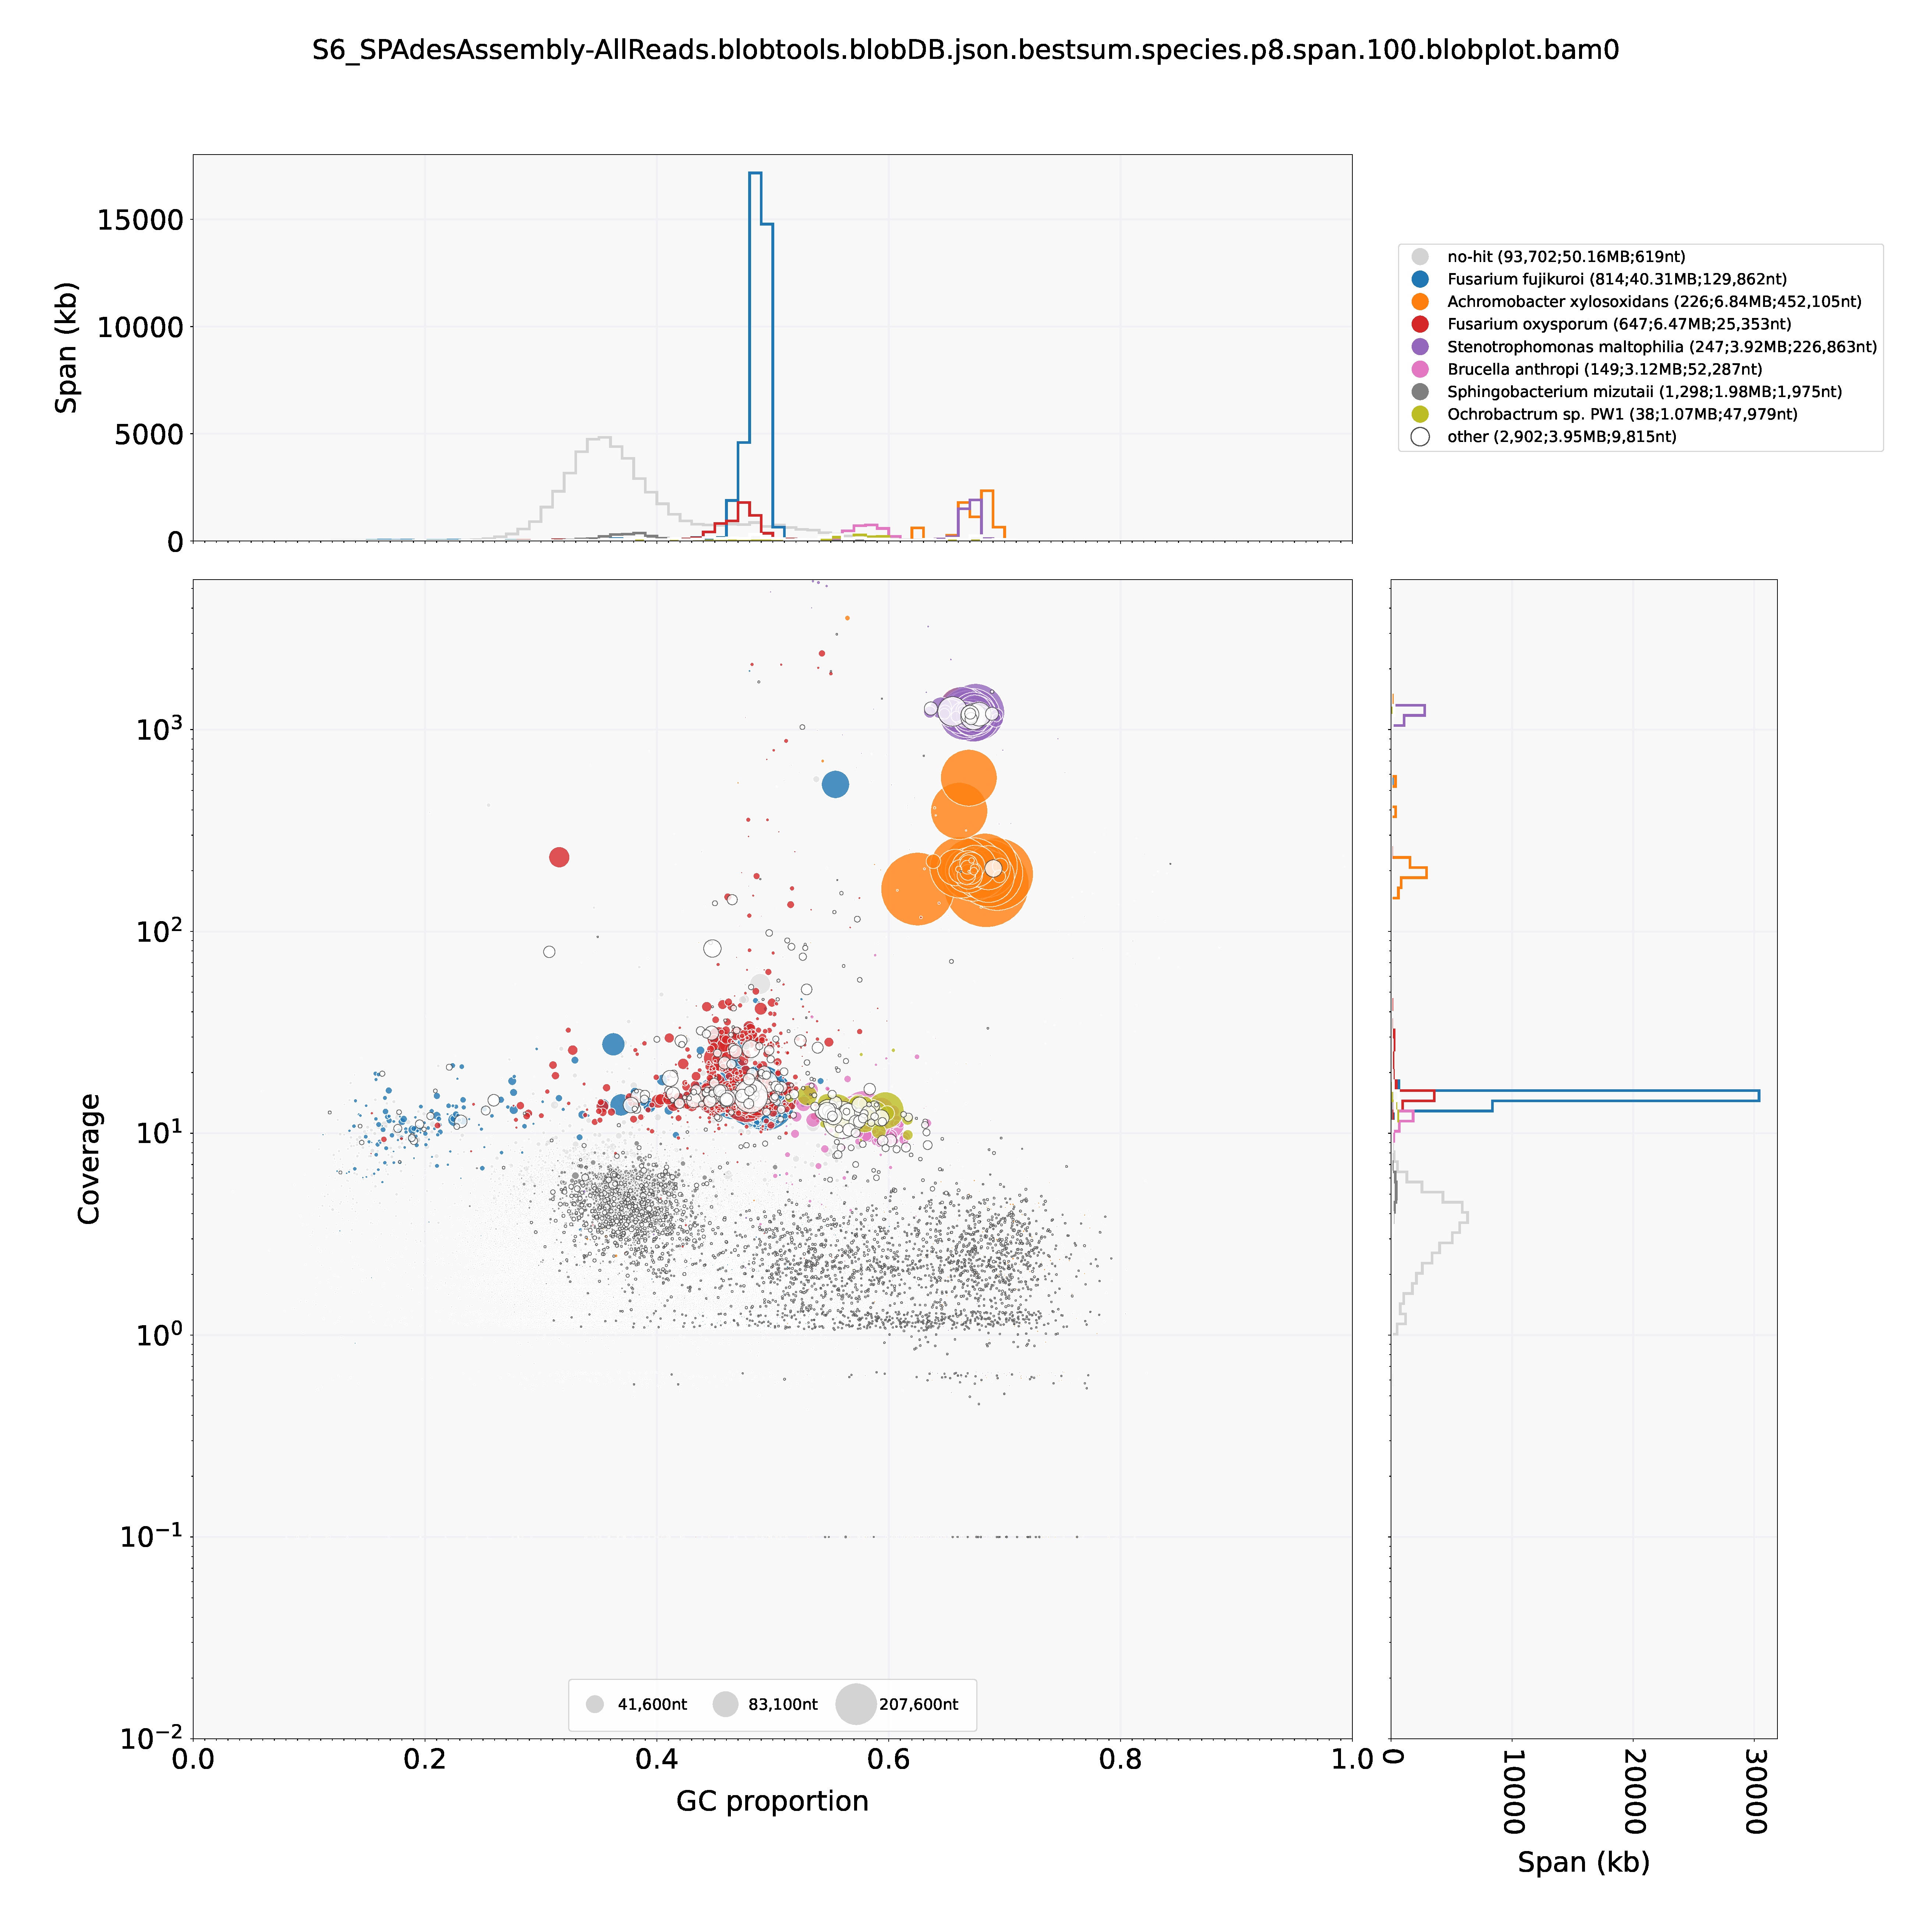
\includegraphics[width=\textwidth]{Appendices/S6_SPAdesAssembly-AllReads.blobtools.blobDB.json.bestsum.species.p8.span.100.blobplot.bam0.pdf}
        \caption{}
        \label{fig:BlobPlot-S6-All}
    \end{subfigure}
    \begin{subfigure}[]{0.9\textwidth}
        \centering
        \includegraphics[width=\textwidth]{Appendices/S6_SPAdesAssembly-AllReads.blobtools.blobDB.json.bestsum.species.p8.span.100.blobplot.read_cov.bam0.pdf}
        \caption{}
        \label{fig:BlobPlot_readcov-S6-All}
    \end{subfigure}
    \caption[BlobTools visualisations of the unfiltered S6 assembly]{\textbf{BlobTools visualisations of the unfiltered S6 assembly shows bacterial contamination.}
        \subref{fig:BlobPlot-S6-All} BlobPlot of S6. Sequences in the unfiltered assembly are depicted as circles, with diameter proportional to sequence length and coloured by taxonomic annotation based on BLASTN (v2.9.0+) of NCBI nt database.
        \subref{fig:BlobPlot_readcov-S6-All} Read coverage plot of the unfiltered S6 assembly. Mapped reads are shown by taxonomic group at the rank of species.}
        \label{fig:S6:BlobToolsAllreads}
\end{figure}
\bigskip

\begin{figure}[hp!]
    \centering
    \begin{subfigure}[]{0.9\textwidth}
        \centering
        \includegraphics[width=\textwidth]{Figures/TNAU_S32_AllContigs.blobtools.blobDB.json.bestsum.species.p8.span.100.blobplot.bam0.png}
        \caption{}
        \label{fig:BlobPlot-S32-All}
    \end{subfigure}
    \begin{subfigure}[]{0.9\textwidth}
        \centering
        \includegraphics[width=\textwidth]{Figures/TNAU_S32_AllContigs.blobtools.blobDB.json.bestsum.species.p8.span.100.blobplot.read_cov.bam0.png}
        \caption{}
        \label{fig:BlobPlot_readcov-S32-All}
    \end{subfigure}
    \caption[BlobTools visualisations of the unfiltered S32 assembly]{\textbf{BlobTools visualisations of the unfiltered S32 assembly shows bacterial contamination.}
        \subref{fig:BlobPlot-S32-All} BlobPlot of S32. Sequences in the unfiltered assembly are depicted as circles, with diameter proportional to sequence length and coloured by taxonomic annotation based on BLASTN (v2.9.0+) of NCBI nt database.
        \subref{fig:BlobPlot_readcov-S32-All} Read coverage plot of the unfiltered S32 assembly. Mapped reads are shown by taxonomic group at the rank of species.}
        \label{fig:S32:BlobToolsAllreads}
\end{figure}
\bigskip

\subsubsection{\acf{rbp2} Phylogeny of \textit{Fusarium} assemblies}

% Please add the following required packages to your document preamble:
% \usepackage{multirow}
% \usepackage{graphicx}
% \usepackage{lscape}
\begin{landscape}
\begin{table}[]
\centering
\captionsetup{width=\linewidth} 
\caption{[\Ac{tnau}\acf{tef} \acf{ncbi} and Fusariod-ID MSLT database searches.]\textbf{Best hits of extracted \acf{tef} sequences from the \acf{tnau} isolate \textit{de novo} assemblies against the Fusariod-ID MSLT database and \ac{ncbi}}}
\label{tab:Tef1-MLSTdb}
\resizebox{\columnwidth}{!}{%
\begin{tabular}{cccc}
\multirow{2}{*}{\textbf{TNAU Isolate Assembly}} & \multicolumn{3}{c}{\textbf{Fusariod-ID MSLT database}}                                     \\ \cline{2-4} 
                                                & Match 1                      & Match 2                      & Match 3                      \\ \hline
\textbf{S6 All reads}                           & \textit{F. oxysporum} Species Complex & \textit{F. oxysporum} Species Complex & \textit{F. oxysporum} Species Complex \\
\textbf{S6 \textit{F. oxysporum}  Reads}                 & \textit{F. oxysporum} Species Complex & \textit{F. oxysporum} Species Complex & \textit{F. oxysporum} Species Complex \\
\textbf{S16}                                    & \textit{F. oxysporum} Species Complex  & \textit{F. oxysporum} Species Complex  & \textit{F. oxysporum} Species Complex  \\
\textbf{S32 All reads}                          & No Matches                   & No Matches                   & No Matches                   \\
\textbf{S32 \textit{F. oxysporum}  Reads}                & No Matches                   & No Matches                   & No Matches                   \\
\textbf{S32 \textit{F. oxysporum}}                        & No Matches                   & No Matches                   & No Matches                  
\end{tabular}%
}
\end{table}
\end{landscape}

\begin{figure}[htp!]
    \centering
    \includegraphics[width=14cm]{Appendices/RPNii-Phylogeny.pdf}
    \caption[\Acl{rbp2} phylogeny of \acl{tnau} \textit{Fusarium} isolates.]{\textbf{\Acl{rbp2} phylogeny of \acl{tnau} \textit{Fusarium} isolates.} \Ac{tnau} isolates S16, S32 and SY-2 sit within the \acf{FFSC} clade. The isolates from \ac{tnau} are shown in red text. The \acf{Fs} clade is shown in pink. \Acf{Focub4} isolates are in blue. \Acf{Focub1} isolates are shown in green. \acf{Focub} isolates with race not recorded are shown in yellow. Percentages represent values from 1000 bootstrap replicates. The tree is rooted through \textit{Fusarium graminearum} PH-1 \ac{rbp2}.}
    \label{fig:rbp2Phylo}
\end{figure}
\bigskip


\clearpage
\section{Appendix B}
\begin{table}[h]
\caption{Reference \ac{mimp} sequences used to build \ac{hmm}}
\label{apx:RefMimps}
\resizebox{\columnwidth}{!}{%
\begin{tabular}{llcc}
\multicolumn{1}{c}{Isolate Source} & \multicolumn{1}{c}{Sequence Name} & Size (bp) & GenBank Accession \\
\textit{Fusarium oxysporum f. sp. lycopersici} & Fusarium oxysporum f. sp. lycopersici MITE mimp4, complete sequence & 220 & EU833101.1 \\
\textit{Fusarium oxysporum f. sp. melonis} & Fusarium oxysporum f. sp. melonis MITE mimp3, complete sequence & 216 & EU833100.1 \\
\textit{Fusarium oxysporum} & Fusarium oxysporum repetitive element mimp2 & 213 & AF076625.1 \\
\textit{Fusarium oxysporum} & Fusarium oxysporum repetitive element mimp1 & 223 & AF076624.1
\end{tabular}%
}
\end{table}

\clearpage
\begin{table}[h]
\caption{Reference set of \acfp{sixg} used for identification of \ac{sixg} homologues in \acl{Fo} genomes. }
\label{apx:sixgenerefs}
\resizebox{\textwidth}{!}{%
\begin{tabular}{lll}
\textit{SIX gene} & Genbank Reference & Isolate \\
\textit{SIX1} & AJ608702.1 & Foly \\
\textit{SIX2} & GQ268949.1 & Foly\_BFOL-51 \\
\textit{SIX3} & AM234063.1 & Foly \\
\textit{SIX4} & GQ268951.1 & Foly\_BFOL-51 \\
\textit{SIX5} & GQ268952.1 & Foly\_BFOL-51\_5 \\
\textit{SIX6} & GQ268953.1 & Foly\_BFOL-51 \\
\textit{SIX7} & GQ268954.1 & Foly\_BFOL-51\_7 \\
\textit{SIX8} & FJ755837.1 & Foly\_007 \\
\textit{SIX9} & KC701447.1 & Foly\_007 \\
\textit{SIX10} & KC701448.1 & Foly\_007 \\
\textit{SIX11} & KC701449.1 & Foly\_007 \\
\textit{SIX12} & KC701450.1 & Foly\_007 \\
\textit{SIX13} & KC701451.1 & Foly\_007 \\
\textit{SIX14} & KC701452.1 & Foly\_007 \\
\textit{SIX15} & KY073750.1 & Foly\_1943
\end{tabular}%
}
\end{table}

\clearpage
\section{Appendix C}
\label{apx:mediaRecipies}

\begin{itemize}
    \item \textbf{\Acf{pdb}}: 24g potato dextrose (Sigma-Aldrich, UK) per L of distilled water.
    \item \textbf{\Acf{pda}}: 24g potato dextrose (Sigma-Aldrich, UK)  and 15g of agar (Sigma-Aldrich, UK) per L of distilled water.  
    \item \textbf{\Acf{ypgb}}: 5g yeast extract (Sigma-Aldrich, UK), 5g peptone (Sigma-Aldrich, UK), and 10g glucose  (Sigma-Aldrich, UK) per L of distilled water. 
    \item \textbf{\Acf{ypgb}}: 5g yeast extract (Sigma-Aldrich, UK), 5g peptone (Sigma-Aldrich, UK), 10g glucose (Sigma-Aldrich, UK), and 15g agar (Sigma-Aldrich, UK) per L of distilled water.
\end{itemize}

\newpage
\label{apx:outliers}

\begin{figure}[hp!]
    \centering
    \includegraphics[width=\textwidth]{Appendices/sum_plot-filtered.pdf}
    \caption[Outliers identified in the dataset] {\textbf{Outliers identified in the dataset.} The sum of all features across samples. Samples C12.1, D15.1, D15.3, D15.4, F12.3, F15.1, F15.3, and F9.4 were identified as outliers and removed from the dataset. The blank samples were also removed from the statistical analysis.} 
    \label{fig:SampleSumPlot}
\end{figure}

\begin{figure}[htp!]
    \centering
    \includegraphics[width=\textwidth]{Figures/AllFeaturesAllSamples_Clustered.png}
    \caption[Heatmap showing hierarchical clustering of samples based on feature peak intensities.]{\textbf{Heatmap showing hierarchical clustering of samples based on 3931 feature peak intensities.} The distance measure was Euclidean and the ward.D algorithm was used for clustering. Class shows the treatment time and group. Value shows the normalised peak intensity. Values show normalised peak intensity. Features were normalised to the sodium formate \ch{Na(NaCOOH)3} adduct ($m/z=226.9521$), log-transformed and scaled (Pareto scaling). Figure generated using MetaboAnalyst (v6.0).}
    \label{fig:AllFeaturesAllSamples}
\end{figure}



\begin{figure}[ph!]
  \centering
  \begin{subfigure}[b]{\textwidth}
    \includegraphics[width=\textwidth]{Figures/FirstTimePointXanthomonasBLQs.pdf}
    \caption{}
    \label{fig:XvmFirstTimeBLQs}
  \end{subfigure}
   \begin{subfigure}[b]{\textwidth}
    \includegraphics[width=\textwidth]{Figures/FirstTimePointFusariumBLQs.pdf}
    \caption{}
    \label{fig:FocFirstTimeBLQs}
  \end{subfigure}
     \begin{subfigure}[b]{\textwidth}
    \includegraphics[width=\textwidth]{Figures/FirstTimePointDroughtBLQs.pdf}
    \caption{}
    \label{fig:DroFirstTimeBLQs}
  \end{subfigure}
     \begin{subfigure}[b]{\textwidth}
    \includegraphics[width=\textwidth]{Figures/FirstTimePointControlBLQs.pdf}
    \caption{}
    \label{fig:ConFirstTimeBLQs}
  \end{subfigure}
  \caption[RGB images of 'Grande Naine' banana plants at the first sample time points.]{\textbf{RGB images of 'Grande Naine' banana plants at the first sample time points.}
  \textbf{\subref{fig:XvmFirstTimeBLQs}}) \acl{xvm}-inoculated plants at 7 \acl{dpi}.
  \textbf{\subref{fig:FocFirstTimeBLQs}}) \acl{Focub4}-inoculated plants at 15 \acl{dpi}.
  \textbf{\subref{fig:DroFirstTimeBLQs}}) Drought-stressed plants at 7 \ac{dpi}, no-watering.
  \textbf{\subref{fig:ConFirstTimeBLQs}}) Mock-inoculated plants at 7 \ac{dpi}.
  Plant labels are provided in white text and correspond to sample labels used in \acl{um} analysis.
  }
  \label{fig:FirstTimePointSymptoms}
\end{figure}

\begin{figure}[ph!]
  \centering
  \begin{subfigure}[b]{\textwidth}
    \includegraphics[width=\textwidth]{Figures/SecondTimePointXanthomonasBLQs.pdf}
    \caption{}
    \label{fig:XvmSecondTimeBLQs}
  \end{subfigure}
   \begin{subfigure}[b]{\textwidth}
    \includegraphics[width=\textwidth]{Figures/SecondTimePointFusariumBLQs.pdf}
    \caption{}
    \label{fig:FocSecondTimeBLQs}
  \end{subfigure}
     \begin{subfigure}[b]{\textwidth}
    \includegraphics[width=\textwidth]{Figures/SecondTimePointDroughtBLQs.pdf}
    \caption{}
    \label{fig:DroSecondTimeBLQs}
  \end{subfigure}
     \begin{subfigure}[b]{\textwidth}
    \includegraphics[width=\textwidth]{Figures/SecondTimePointControlBLQs.pdf}
    \caption{}
    \label{fig:ConSecondTimeBLQs}
  \end{subfigure}
  \caption[RGB images of 'Grande Naine' banana plants at the second sample time points.]{\textbf{RGB images of 'Grande Naine' banana plants at the second sample time points.}
  \textbf{\subref{fig:XvmSecondTimeBLQs}}) \acl{xvm}-inoculated plants at 10 \acl{dpi}.
  \textbf{\subref{fig:FocSecondTimeBLQs}}) \acl{Focub4}-inoculated plants at 18 \acl{dpi}.
  \textbf{\subref{fig:DroSecondTimeBLQs}}) Drought-stressed plants at 10, no-watering.
  \textbf{\subref{fig:ConSecondTimeBLQs}}) Mock-inoculated plants at 10 \ac{dpi}.
  Plant labels are provided in white text and correspond to sample labels used in \acl{um} analysis.
  }
  \label{fig:SecondTimePointSymptoms}
\end{figure}

\begin{figure}[ph!]
  \centering
  \begin{subfigure}[b]{\textwidth}
    \includegraphics[width=\textwidth]{Figures/ThirdTimePointXanthomonasBLQs.pdf}
    \caption{}
    \label{fig:XvmThirdTimeBLQs}
  \end{subfigure}
   \begin{subfigure}[b]{\textwidth}
    \includegraphics[width=\textwidth]{Figures/ThirdTimePointFusariumBLQs.pdf}
    \caption{}
    \label{fig:FocThirdTimeBLQs}
  \end{subfigure}
     \begin{subfigure}[b]{\textwidth}
    \includegraphics[width=\textwidth]{Figures/ThirdTimePointDroughtBLQs.pdf}
    \caption{}
    \label{fig:DroThirdTimeBLQs}
  \end{subfigure}
     \begin{subfigure}[b]{\textwidth}
    \includegraphics[width=\textwidth]{Figures/ThirdTimePointControlBLQs.pdf}
    \caption{}
    \label{fig:ConThirdTimeBLQs}
  \end{subfigure}
  \caption[RGB images of 'Grande Naine' banana plants at the third sample time points.]{\textbf{RGB images of 'Grande Naine' banana plants at the third sample time points.}
  \textbf{\subref{fig:XvmThirdTimeBLQs}}) \acl{xvm}-inoculated plants at 13 \acl{dpi}.
  \textbf{\subref{fig:FocThirdTimeBLQs}}) \acl{Focub4}-inoculated plants at 21 \acl{dpi}.
  \textbf{\subref{fig:DroThirdTimeBLQs}}) Drought-stressed plants at 13 days no-watering.
  \textbf{\subref{fig:ConThirdTimeBLQs}}) Mock-inoculated plants at 13 \ac{dpi}.
  Plant labels are provided in white text and correspond to sample labels used in \acl{um} analysis.
  }
  \label{fig:ThridTimePointSymptoms}
\end{figure}


\newpage
\begin{figure}[htp!]
    \centering
    \includegraphics[width=\textwidth]{Appendices/Sig453FeaturesRedSamplesRedGroups.pdf}
    \caption[Heatmap showing hierarchical clustering of samples based on 453 normalised significant feature peak intensities (p ≤ 0.05) (negative mode)]{\textbf{Heatmap showing hierarchical clustering of samples based on 453 normalised significant feature peak intensities (p ≤ 0.05) (negative mode).} The distance measure was Euclidean and the ward.D algorithm was used for clustering. Class shows the treatment time and group. Value shows the normalised peak intensity. Values show normalised peak intensity. Features were normalised to the sodium formate \ch{Na(NaCOOH)3} adduct, log-transformed and scaled (Pareto scaling). Figure generated using MetaboAnalyst (v6.0).}
    \label{fig:Sig543FeaturesNegMode}
\end{figure}

\newpage
\begin{figure}[htp!]
    \centering
    \includegraphics[width=\textwidth]{Appendices/Sig56FeaturesRedSamplesFirstTimePointOnly-ExcludingQCs.png}
    \caption[Heatmap showing hierarchical clustering of samples based on 56 normalised significant feature peak intensities (p ≤ 0.05) from the first time point (negative mode)]{\textbf{Heatmap showing hierarchical clustering of samples based on 56 normalised significant feature peak intensities (p ≤ 0.05) from the first time point (negative mode).} The distance measure was Euclidean and the ward.D algorithm was used for clustering. Class shows the treatment group. Value shows the normalised peak intensity. Values show normalised peak intensity. Features were normalised to the sodium formate \ch{Na(NaCOOH)3} adduct, log-transformed and scaled (Pareto scaling). Figure generated using MetaboAnalyst (v6.0).}
    \label{fig:Sig56FeaturesNegMode}
\end{figure}

\newpage
\begin{figure}[htp!]
    \centering
    \includegraphics[width=\textwidth]{Appendices/RedSamplesSecondTimePoint-NonParametric-ExcludingQCs_heatmap_2_dpi72.pdf}
    \caption[Heatmap showing hierarchical clustering of samples based on 806 normalised significant feature peak intensities (p ≤ 0.05) from the first time point (negative mode)]{\textbf{Heatmap showing hierarchical clustering of samples based on 806 normalised significant feature peak intensities (p ≤ 0.05) (non-parametric ANOVA) from the first time point (negative mode).} The distance measure was Euclidean and the ward.D algorithm was used for clustering. Class shows the treatment group. Value shows the normalised peak intensity. Values show normalised peak intensity. Features were normalised to the sodium formate \ch{Na(NaCOOH)3} adduct, log-transformed and scaled (Pareto scaling). Figure generated using MetaboAnalyst (v6.0).}
    \label{fig:Sig806FeaturesNegMode}
\end{figure}

\end{appendices}

\end{document}                       
%% Done.

